\documentclass[11pt]{article}

% ---------- Encoding & fonts ----------
\usepackage[utf8]{inputenc}
\usepackage[T1]{fontenc}
% Linux Libertine: modern, readable academic serif. Pairs well with the
% Biolinum sans-serif for headings. Much easier on the eye than Latin
% Modern at body sizes for dense empirical prose.
\usepackage{libertine}
\usepackage[libertine]{newtxmath}
\renewcommand*\familydefault{\rmdefault}
\usepackage{microtype}

% Slightly looser line spacing for readability (was default tight).
\linespread{1.08}

% ---------- Layout ----------
\usepackage[margin=1in]{geometry}
\usepackage{setspace}
\usepackage{parskip}

% ---------- Math ----------
% Note: newtxmath (loaded above with libertine) provides AMS-style
% symbols (\Bbbk, etc.) and proofs already. Loading amssymb or amsthm
% on top causes "command already defined" errors. Only amsmath is needed.
\usepackage{amsmath}

% ---------- Figures & tables ----------
\usepackage{graphicx}
\graphicspath{{figures/}}
\usepackage{booktabs}
\usepackage{array}
\usepackage{multirow}
\usepackage{caption}
\usepackage{subcaption}
% float package provides [H] = "place here, exactly, no migration"
\usepackage{float}

% Generous spacing around floats so figures/tables don't crowd prose.
\setlength{\textfloatsep}{16pt plus 3pt minus 3pt}  % between floats and main text
\setlength{\floatsep}{14pt plus 3pt minus 3pt}      % between consecutive floats
\setlength{\intextsep}{14pt plus 3pt minus 3pt}     % around floats placed inline ([h])
\captionsetup{%
  skip=8pt,
  font=small,
  labelfont=bf,
  justification=justified,       % uniform: left-aligned with right-fill
  singlelinecheck=false,         % don't auto-center single-line captions
}

% Allow more aggressive float placement: LaTeX considers more pages and
% never delays a float past the end of its section.
\usepackage{placeins}                               % provides \FloatBarrier
\renewcommand{\topfraction}{0.85}                   % up to 85% of page for top floats
\renewcommand{\bottomfraction}{0.65}
\renewcommand{\textfraction}{0.10}                  % require at least 10% of page for text
\renewcommand{\floatpagefraction}{0.75}
\setcounter{topnumber}{3}                           % up to 3 floats at top of a page
\setcounter{bottomnumber}{2}
\setcounter{totalnumber}{5}

% ---------- Diagrams & plots ----------
\usepackage{tikz}
\usetikzlibrary{arrows.meta, positioning, shapes.geometric, fit, calc,
                backgrounds, decorations.pathreplacing, shadows.blur}
\usepackage{pgfplots}
\pgfplotsset{compat=1.18}
\usepgfplotslibrary{groupplots, statistics, fillbetween}

% ---------- Code & verbatim ----------
\usepackage{listings}
\usepackage{xcolor}
\lstset{
  basicstyle=\ttfamily\small,
  breaklines=true,
  frame=single,
  showstringspaces=false,
  captionpos=b,             % caption always BELOW the listing (matches figure convention)
  abovecaptionskip=6pt,     % consistent spacing above the caption
  belowcaptionskip=4pt,     % consistent spacing below the caption
  aboveskip=10pt,           % consistent space between prose and listing
  belowskip=10pt,
}

% ---------- Accent palette ----------
% Deep teal as primary accent (clinical-modern, distinctive but not loud).
% Used for rules, callout borders, links, and section underlines.
\definecolor{accent}{HTML}{1F5F5B}
\definecolor{accentLight}{HTML}{E6EFEE}
\definecolor{accentDark}{HTML}{143F3C}
\definecolor{warmGray}{HTML}{4A4A4A}
\definecolor{paleGray}{HTML}{F7F7F5}

% Qualitative palette for conditions, grouped by purpose so color
% encodes family (a reader decodes the chart before reading the legend).
% Anchors (A, B):           muted grays
% Primary (C, D, E):        blues, increasing saturation
% Exploratory (B', B'+E):   warm earth tones
% Diagnostic (reactive):    accent teal
\definecolor{condA}{HTML}{B0B0B0}
\definecolor{condB}{HTML}{4A4A4A}
\definecolor{condC}{HTML}{9DC3E6}
\definecolor{condD}{HTML}{4F81BD}
\definecolor{condE}{HTML}{1F4E79}
\definecolor{condBprime}{HTML}{D9A066}
\definecolor{condBprimeE}{HTML}{B45A1F}
\definecolor{condReactive}{HTML}{1F5F5B}

% ---------- Fancy boxes for callouts ----------
\usepackage[most]{tcolorbox}

% Abstract box: plain outlined rectangle, white background, thin border.
% NOT breakable -- if it can't fit on the current page, the whole box moves
% to the next page rather than splitting across a page break.
\newtcolorbox{abstractbox}{%
  enhanced,
  colback=white,
  colframe=warmGray,
  boxrule=0.6pt,
  arc=0pt,
  outer arc=0pt,
  left=14pt, right=14pt, top=12pt, bottom=12pt,
  fontupper=\normalsize,
}

% Key findings highlight box: bolder, used once on page 1.
% NOT breakable -- moves to next page as a unit rather than splitting.
\newtcolorbox{findingsbox}{%
  enhanced,
  colback=accentLight,
  colframe=accent,
  boxrule=1pt,
  arc=3pt,
  outer arc=3pt,
  left=14pt, right=14pt, top=10pt, bottom=10pt,
  title=\textbf{Key Findings},
  coltitle=white,
  colbacktitle=accent,
  fonttitle=\bfseries\large,
  attach boxed title to top left={xshift=8pt, yshift=-8pt},
  boxed title style={
    colback=accent,
    colframe=accent,
    arc=2pt,
    boxrule=0pt,
    left=8pt, right=8pt, top=2pt, bottom=2pt,
  },
}

% ---------- Citations ----------
% Numeric citation style ([1], [2], ...) -- more compact and standard in
% ML/clinical-AI venues; reduces in-line text density.
\usepackage[numbers, square, sort&compress]{natbib}
% xurl allows long URLs in the bibliography to break at any character,
% preventing overflow into the margin. Must be loaded before hyperref.
\usepackage{xurl}
\usepackage{hyperref}
\hypersetup{
  colorlinks=true,
  linkcolor=accentDark,
  citecolor=accentDark,
  urlcolor=accentDark,
  pdftitle={Procedural Input Verification for Clinical Tool Calling: An Empirical Study of Interwhen-Style Verifier-Guided Reasoning with LLM-Extracted References},
  pdfauthor={Jack Yang, Jaeyoon Wang, Aly Moosa},
  pdfsubject={Verifier-guided reasoning for clinical decision support, applied to medical-calculator tool calls},
  pdfkeywords={clinical AI, procedural input verification, verifier-guided reasoning, interwhen, reactive extraction, fact extraction, medical calculators, KARMA, Model Context Protocol, LLM evaluation},
}

% ---------- Custom commands ----------
% Keywords block under the abstract (article class doesn't ship one).
\providecommand{\keywords}[1]{%
  \vspace{0.5em}\noindent\textbf{Keywords:} #1\par
}

% Semantic identifier styling. Use \toolname{} for tool names, schema
% identifiers, file paths in flowing prose -- renders as italic so the
% text breaks naturally at line ends (unlike \texttt{} which is rigid
% monospace and causes overfull hboxes on long names). Reserve \texttt{}
% only for short literal code values in prose (e.g., \texttt{sex=1}).
\newcommand{\toolname}[1]{\textit{#1}}

% ---------- Cross-references ----------
\usepackage{cleveref}

% ---------- Section heading styling ----------
% Sans-serif headings (Biolinum, ships with libertine) — visually
% distinct from the serif body, easier to scan, lighter than serif bold.
\usepackage{titlesec}
\titleformat{\section}
  {\sffamily\Large\bfseries\color{accent}}
  {\thesection}{0.6em}{}
\titleformat{\subsection}
  {\sffamily\large\bfseries\color{accentDark}}
  {\thesubsection}{0.6em}{}
\titleformat{\subsubsection}
  {\sffamily\normalsize\bfseries}
  {\thesubsubsection}{0.6em}{}

% ---------- Custom title block ----------
% Replaces \maketitle with a distinctive layout: large title, thick
% accent rule, author / affiliation / date in a clean three-line block.
%
% Note on \and: standard LaTeX \maketitle uses a tabular under the hood,
% so \and expands to a tab mark (&). Our custom title is plain text, so
% we locally redefine \and to render as a comma-space separator. This
% keeps `\author{A \and B \and C}` working both ways.
% Subject tag and affiliation rendered in the title block. Override
% either with \renewcommand{...} in main.tex if needed.
\makeatletter
\newcommand{\@subject}{Artificial intelligence
                       \,$\cdot$\, Intermediate-step verification
                       \,$\cdot$\, Medical informatics}
\newcommand{\@affiliation}{}   % empty by default; set in main.tex

\renewcommand{\maketitle}{%
  \begingroup
  \renewcommand{\and}{\unskip,\ \ignorespaces}%
  \noindent
  {\color{accent}\rule{\linewidth}{0.4pt}}\par
  \vspace{12pt}
  \noindent{\sffamily\LARGE\bfseries\@title\par}
  \vspace{8pt}
  \noindent{\sffamily\small\itshape\color{accent}\@subject\par}
  \vspace{12pt}
  \noindent{\sffamily\large\@author\par}
  \ifx\@affiliation\@empty\else
    \vspace{3pt}
    \noindent{\sffamily\small\itshape\color{warmGray}\@affiliation\par}
  \fi
  \vspace{4pt}
  \noindent{\sffamily\small\color{warmGray}\@date\par}
  \vspace{4pt}
  \noindent{\color{accent}\rule{\linewidth}{0.4pt}}\par
  \vspace{20pt}
  \endgroup
}
\makeatother


\title{Procedural Input Verification for Clinical Tool Calling:\\
An Empirical Study of Interwhen Verifier-Guided Reasoning with LLM-Extracted References}

\author{Jack Yang \and Jaeyoon Wang \and Aly Moosa}
\makeatletter
\renewcommand{\@affiliation}{Bill \& Melinda Gates Foundation}
\makeatother

\date{\today}

\begin{document}
\maketitle

% ── Boxed abstract (custom callout style) ─────────────────────────────────
\begin{abstractbox}
\noindent\textbf{\color{accent}Abstract.}\quad
% =============================================================================
% ABSTRACT — design narrative is current (9-condition, best-practice). Only the
% headline-results paragraph is TBD; fill it after the primary study rerun:
%   (1) does verifier-guided extraction beat B' under schema-gating + query
%       intervention + abstention? (2) does placement (upfront vs reactive)
%       carry the effect? (3) do citations or k-shot close any residual gap?
% Bonferroni n = 6; per-test alpha = 0.00833.
% =============================================================================

Verifier-guided reasoning (interwhen-style) intercepts an LLM's intermediate
reasoning steps and asks an external verifier to approve them before they
take effect. We evaluate this mechanism in a clinical decision-support
setting --- specifically, \emph{procedural input verification} of tool-call
payloads against patient facts extracted from case vignettes --- using
medical\_calculator\_eval ($N=1066$) and Qwen3-30B-A3B-Thinking-2507 as the
primary model. The verifier compares each (field, value) pair the model
proposes to dispatch to an MCP medical calculator against a reference set
of facts extracted from the case by Sonnet 4.6.

We study a single experimental factor, the architecture of the
input-verification pipeline, across four primary conditions presented at
their best-practice configuration (schema-gated verifier comparison,
query-style intervention prompts, prompt-only calibrated abstention).
The four conditions span three orthogonal axes: extraction placement
(upfront full-schema vs reactive per-tool-call), output format (bare
values vs citation-anchored pairs), and sampling ($k=1$ vs $k=3$ majority
vote). Six paired McNemar contrasts are pre-registered at family
$\alpha=0.05$ (Bonferroni-corrected per-test $\alpha=0.00833$).

The apparatus gate held (Sonnet on B reached $80.4\%$, within $\pm 3$
pp of the published $81.9\%$ reference). Accuracy is driven by tool use,
not by verification: it rises from $41.6\%$ without tools (A) to
$50.3\%$ with tools (B) to $71.6\%$ when tool use is forced (B$'$; both
$p_{\text{Bonf}} < 10^{-9}$). \textbf{None of the four
verifier-guided extractor pipelines improved on B$'$}: all landed
within $0.9$ pp ($72.0$--$72.5\%$), and no pre-registered contrast
against B$'$ reached significance. Extraction placement, citation
grounding, and $k=3$ voting each had no measurable effect, though
reactive extraction matched upfront accuracy at $\sim$$40\%$ of the
token cost. The null is informative: the identical mechanism
\emph{harmed} accuracy when un-gated (pilot diagnostics), so
best-practice hygiene removes that harm and returns the verifier to
parity with B$'$ rather than adding value on top of it. The binding
constraint is the LLM-extracted reference layer, not the verifier
mechanism --- procedural input verification helps only as much as the
reference it is given is correct.

\end{abstractbox}

\vspace{8pt}

% ── Key Findings highlight box ────────────────────────────────────────────
\begin{findingsbox}
\begin{itemize}\setlength\itemsep{3pt}
  \item \textbf{Procedural input verification did not improve clinical
        tool-call accuracy.} Across four pre-registered primary contrasts
        (Bonferroni $\alpha=0.0125$), no verifier condition (E, D, C)
        significantly beat the no-verifier baseline B.
  \item \textbf{Under a tool-forcing system prompt the verifier
        \emph{actively hurt} accuracy by 9.0 pp} (McNemar $p < 10^{-15}$).
        118 vignettes flipped from correct to wrong; only 22 flipped the
        other way.
  \item \textbf{The harm came from the reference, not the verifier.}
        A single field (sex) accounted for $\sim$32\% of all flags
        under upfront full-schema extraction, despite being among the
        easiest fields to extract correctly --- implicating the
        extraction \emph{architecture}, not the verifier's comparison logic.
  \item \textbf{Reactive per-tool-call extraction \emph{partially}
        recovered the diagnostic markers but not accuracy.} Sex fell to
        13\% of flags, correct-rate on intervention rows doubled, and
        total token cost dropped $\sim$57\%, but the accuracy gain vs
        upfront B$'$+E was not significant ($+1.9$ pp, $p = 0.103$).
        Schema size is a contributor, not the sole bottleneck.
\end{itemize}

\end{findingsbox}

\vspace{8pt}

\keywords{clinical AI safety, procedural input verification, verification, interwhen, large language models, reasoning trace, fact extraction, medical calculators, KARMA, Model Context Protocol, agent evaluation}

\vspace{12pt}

\section{Introduction}
\subsection{Motivation: Wrong Inputs Defeat Correct Calculators}
\label{sec:intro_motivation}

Clinical decision-support is increasingly delivered by large language
models (LLMs) that call deterministic backend tools --- risk calculators,
dosing engines, eligibility checks --- via a structured tool-calling
interface. The deterministic backend is the easy part: a correctly
implemented CHA\textsubscript{2}DS\textsubscript{2}-VASc calculator
returns the right score on any input. The hard part is the boundary
where the LLM hands the calculator its inputs. A correct calculator
called with a transposed creatinine value, the wrong patient sex, or a
miscoded comorbidity will return a plausible-but-wrong answer that no
amount of downstream verification of the textual response can detect.

Concretely, in the medical\_calculator\_eval benchmark used in this study,
many vignettes admit only one ``correct'' calculator and one ``correct''
input mapping. A model that names the right calculator but misreads
the patient's sex from the case will receive a confidently wrong score
and present it as the answer. The failure mode is structural: it lives
at the LLM-to-tool input boundary, not in the calculator and not in
the final textual summary.

\subsection{Scope: Procedural Input Verification}
\label{sec:intro_scope}

We study \emph{procedural input verification} of tool calls: an
intermediate intervention that inspects the JSON payload the LLM sends
to a deterministic clinical calculator \emph{before} the calculator
runs. This is distinct from output verification (re-checking the final
textual answer), end-to-end outcome verification (was the diagnosis
right?), and retrieval grounding (was the cited fact in the source?).
The verification fires at one specific point in the agent loop: between
the model emitting a \verb|<tool_call>| block and the MCP tool being
invoked. The verifier compares each (field, value) pair the model
proposes to dispatch against an independently extracted reference set
of patient facts. If the case (and the extractor) say sex = female and
the model proposes sex = male, the call is flagged and the model is
asked to revise before the calculator runs.

This is the scope of every claim in this paper. We do not study other
verification surfaces, and our results say nothing about them directly.

\subsection{The Verification Hypothesis}
\label{sec:intro_hypothesis}

We study a single experimental factor: the architecture of the
input-verification pipeline. Four primary hypotheses are
pre-registered, one per architectural axis (\cref{sec:methods_stats}):

\textbf{H1 (placement).} Best-practice procedural input verification
with upfront full-schema extraction improves accuracy over the
forced-tool baseline B$'$.

\textbf{H2 (placement).} Best-practice procedural input verification
with reactive per-tool-call extraction improves accuracy over B$'$.

\textbf{H3 (output format).} Adding citation grounding to the
reactive pipeline (\texttt{value} + verbatim source span) improves
accuracy over the bare-value reactive baseline.

\textbf{H4 (sampling).} Replacing single-sample reactive extraction
with $k=3$ majority voting improves accuracy over the single-sample
reactive baseline.

``Best-practice'' here means schema-gated verifier comparison,
query-style intervention prompts, and prompt-only calibrated
abstention --- the three hygiene properties baked into all primary
study conditions (\cref{sec:methods_prereg}). These properties are
not factors under test; they were motivated by pilot diagnostics
(\cref{sec:methods_pilots}) and are held constant across H1--H4.

\subsection{Contributions and Roadmap}
\label{sec:intro_contributions}

This paper contributes the following. (i) A nine-condition evaluation
of procedural input verification on a clinical tool-calling benchmark
under a best-practice pre-registered design that varies only the
extractor pipeline across the four primary study conditions.
(ii) Six pre-registered McNemar contrasts (Bonferroni
$\alpha = 0.00833$) testing four hypotheses about extractor
architecture: placement (upfront vs reactive), output format (bare vs
citation-anchored), and sampling ($k=1$ vs $k=3$ majority vote).
(iii) A pilot-diagnostic methodology section that documents the
un-gated and correction-style variants that motivated the
best-practice hygiene baked into the primary study, including a
58.6\% non-required-field flag rate under un-gated extraction.
(iv) A uniform per-condition logging schema and analysis surface that
makes the four extractor pipelines directly comparable on accuracy,
flag composition, and cost.

We do \emph{not} claim that interwhen ``does not work.'' Our results
adapt the mechanism to a setting where the verifier's reference must be
an independent fact set extracted from the case --- a ground-truth
reference layer that interwhen's trace-state extraction does not have to
produce --- and the binding constraint, if one remains under
best-practice configuration, is jointly that reference pipeline and the
verifier's comparison surface.

The rest of the paper is organized as follows. \Cref{sec:bg_interwhen}
reviews the interwhen mechanism and the clinical-tool-calling setting.
\Cref{sec:methods_benchmark} describes the apparatus, the nine
conditions, the pre-registered configuration, and the statistical
analysis. \Cref{sec:results_gate} reports the apparatus gate and the
six pre-registered contrasts;
\cref{sec:results_architecture,sec:results_diagnostic} develop the
within-architecture comparisons and the post-hygiene flag
composition. \Cref{sec:disc_summary} synthesizes what the results
show and the implications for deploying intermediate verification in
clinical AI.


\section{Background}
\subsection{Verifier-Guided Reasoning (Interwhen)}
\label{sec:bg_interwhen}

Interwhen~\citep{bhat2026interwhen} is a verifier-guided reasoning
framework in which a monitor periodically polls an LLM's reasoning
trace, forks the model to extract verifiable state from the partial
trace, and runs verifiers on that state asynchronously --- injecting
feedback and re-prompting only when a violation is detected. The
verifiers are code-based predicates over partial traces and can be
synthesized automatically from natural-language policy documents,
including provably correct variants in Lean and z3. Interwhen is
evaluated across both non-agentic reasoning (math, logic) and agentic
tool-calling benchmarks (e.g., $\tau^2$-bench). Crucially for our
adaptation, the state the verifier consumes is itself recovered by an
LLM extraction step over the trace, and interwhen explicitly analyzes
the framework's robustness to errors in that extraction.

We adapt the mechanism rather than re-implement it, preserving
interwhen's verify/fix control flow exactly --- on flag, inject
feedback and re-prompt; on clean, dispatch the tool and continue.
Three things change. First, instead of polling the trace at intervals,
we fix the intercept at a single deterministic commit point: the
moment the primary model emits a \verb|<tool_call>| block, whose parsed
JSON is the state under check. Second, the LLM extraction reads the
patient \emph{case} --- the task input --- rather than the model's own
reasoning trace; interwhen recovers the model's asserted state from the
trace and checks it against a policy, whereas we recover an independent
reference from the case and check the model's proposed inputs against
it. Third, in place of a policy-synthesized verifier we use a
hand-built deterministic field-by-field comparator. The transport also
differs: we use vLLM's text-completions endpoint with a custom
synchronous loop driver rather than the streaming variant, because the
primary model is served behind a standard completions API.

\subsection{Clinical Tool-Calling and KARMA}
\label{sec:bg_karma}

KARMA~\citep{karma2024} is a structured evaluation framework for medical
AI published by EkaCare. We use its publicly released
medical\_calculator\_eval benchmark ($N=1066$ vignettes spanning 24
calculator categories, from cardiology to obstetrics) and the
associated MedAI Model Context Protocol (MCP)
toolset~\citep{medai_mcp}.

The MCP toolset exposes six meta-tools, of which three are central to
this study:
\toolname{medical\_calculator\_list} enumerates available calculators;
\toolname{medical\_calculator\_input} returns the JSON Schema for a chosen
calculator's input; and \toolname{medical\_calculator\_output} dispatches the
calculator with an \verb|input_data| payload. Each calculator carries a
typed JSON Schema with enums, ranges, and field descriptions. The union
of input field names across all calculators yields a vocabulary of
$\sim$500 unique fields. This union is the reference vocabulary the
verifier and extractor share, by construction --- both consume the
schemas EkaCare ships, so neither can refer to a field the other does
not know about.

\subsection{Verification Surfaces: Where to Intervene}
\label{sec:bg_surfaces}

LLM-driven clinical AI admits intervention at several surfaces, which
are often conflated in casual discussion. We distinguish:

\textit{Input verification} (this paper). The verifier inspects the
model's proposed tool-call arguments \emph{before} dispatch. Catches
wrong inputs at the boundary where they would otherwise propagate
into a deterministic backend. Fires at intermediate commit points;
firing frequency scales with tool-call rate.

\textit{Output verification.} The verifier reads the model's final
textual answer and may request revision. Cannot catch a wrong tool
input that produced a confidently-stated wrong answer unless the
final text exposes the inconsistency. Condition D in our study is the
closest output-style comparator.

\textit{Grounding / retrieval-augmented verification.} The reference
is retrieved text. A different problem class --- the question becomes
``is the claim supported by retrieved evidence?'' rather than ``is the
proposed input consistent with the case?'' Not evaluated here.

\textit{Self-verification.} The model is asked, in-prompt, to check
itself. No external reference. Condition C is our control for ``is any
external machinery necessary?''

This paper concerns the first surface. Every claim about ``the
verifier'' refers to procedural input verification specifically.

Procedural input verification is a \emph{special case} of
reasoning-trace verification: the model's tool-call emission is one
step in its trace, and we intercept at that step. What distinguishes
our setting is where the verifier's reference comes from and where the
commit point sits. Interwhen recovers verifiable state by polling the
trace at intervals; in a clinical agent most of that trace is
unstructured prose, and the reference the verifier needs --- the
patient's actual values --- is not in the trace at all but in the case
text. The model's typed tool-call payload is the first point in the
trace where a machine-checkable structured commit exists, and the
calculator's input schema defines exactly what fields constitute that
commit. A flag therefore
localizes to a specific (calculator, field, value) tuple --- auditable
in the way clinical safety reviews require. Second, existing clinical
decision-support pipelines already \emph{have} these tool boundaries
(risk calculators, formularies, eligibility checkers, FHIR queries),
so input verification inserts at a place the deployment architecture
already exposes, rather than requiring the workflow to be restructured
around inline reasoning checks.

\subsection{The Reference-Extraction Problem}
\label{sec:bg_reference}

A subtlety in the clinical adaptation deserves explicit attention:
\emph{the reference itself must come from somewhere}. Interwhen already
relies on an LLM to extract the verifier's input variables, but it
extracts them from the model's own reasoning trace --- the state the
verifier checks is the model's asserted state, scored against a policy.
In our setting the verifier instead needs the patient's true values,
which live only in the natural-language case. Before the verifier can
compare anything, the case must be parsed into field--value pairs by an
LLM, and that extracted record is then treated as the reference against
which the model's proposed inputs are judged. The model-based
extraction step is therefore not new to interwhen; what is new is that
it now stands between the case and the verifier as the source of ground
truth, which is where the verifier's safety guarantee can weaken.

We use an external LLM of a different model family than the primary
to produce the reference (specific model, version, and serving
configuration in \cref{sec:methods_benchmark}). The cost of this
design is that the extractor is itself an LLM, with its own
distribution of errors. This paper's main finding is that those
errors --- not the verifier mechanism --- bound the achievable
accuracy.

\subsection{Which Failure Classes Input Verification Can Reach}
\label{sec:bg_scope}

EkaCare's own error analysis of
medical\_calculator\_eval~\citep{ekacare_error_analysis} identifies two
failure classes that persist even with tool access. The first is
\emph{wrong calculator selected} --- the model picks a semantically
adjacent but distinct tool (e.g., a generic BMI calculator where a
sex-specific variant is required). The second, affecting 12--13\% of
samples across the three models they evaluated, is \emph{right
calculator, wrong inputs}, which decomposes into (a) enum misselection
(mapping ``sedentary'' to ``very\_active'' in a TDEE activity field)
and (b) unit-conversion overreach, where the model receives a correct
calculator result and then rewrites it into a different unit,
introducing an error the calculator did not make.

Procedural input verification is scoped to exactly one of these
sub-classes. It fires before dispatch on the tool-call payload, so it
can catch enum misselection and analogous wrong-input errors at the
boundary --- sub-class (a) above. It \emph{cannot} reach sub-class (b):
unit-conversion overreach occurs after the calculator returns, on the
output surface, where only a post-hoc check such as Condition D could
intervene. Wrong-calculator selection is likewise out of scope --- the
verifier checks field values for the calculator the model has already
chosen, not the choice of calculator itself. The addressable ceiling
for the primary study conditions is therefore the enum/wrong-input
portion of the 12--13\% band, not the full band; we report the split
where the logs permit and calibrate expected effect sizes accordingly.
Condition D is the only arm positioned to reach the unit-overreach
sub-class, and it targets a different failure than the B$'$+E
conditions rather than a more thorough version of the same one.


\section{Methods}
\subsection{Benchmark and Primary Model}
\label{sec:methods_benchmark}

The benchmark is medical\_calculator\_eval (Hugging Face dataset
\textit{ekacare/medical\_calculator\_eval}, test split, $N=1066$
vignettes), released by EkaCare as part of the KARMA evaluation
framework~\citep{karma2024}. We use the public release without
modification.

Each item is a single-turn task: a case-narrative vignette in
natural-language prose, a target calculator, an \emph{expected
numerical value} for a designated primary output field, and a
per-item tolerance. There is no conversation --- the model receives
the vignette once and produces a single response. Each item also
carries a per-row \emph{confinement instruction} --- a prompt suffix
that instructs the model to reply with a single JSON object
containing the primary field --- which the adapter appends to the
vignette before generation. Scoring is binary: the harness extracts a
numerical prediction from the model's reply (preferring fenced JSON
blocks, falling back to the last number in the text), and the item is
marked correct iff
$|\text{predicted} - \text{expected}| \le \text{tolerance}$. Parse
failures and missing-field responses score as wrong. All accuracy
numbers in this paper are this strict tolerance-based binary
correctness, not partial-credit scores. Critically, the input is
free-text prose rather than structured fields --- the reason an LLM
extractor is required to populate the verifier's reference at all.
Structured-input benchmarks (e.g., EHR-keyed inputs) would remove
the extraction bottleneck this paper diagnoses. Curation details
(vignette authorship, validation, calculator coverage) are documented
in the KARMA release. The primary model under evaluation is
Qwen3-30B-A3B-Thinking-2507~\citep{qwen3_thinking}, served via
vLLM~\citep{vllm2023} on the text-completions endpoint with
temperature $0.0$, top-$p$ $1.0$, max generation length $4096$ tokens,
and a tool-calling loop bounded at $10$ turns. The primary model's
sampling is deterministic by construction (temperature zero, frozen
MCP schema dump). The extractor's sampling varies by condition and
is documented in \cref{sec:methods_prereg}.

The fact extractor used in all extractor-enabled conditions is Claude
Sonnet 4.6~\citep{claude_sonnet_4_6}, called with a single pinned
model snapshot for the duration of each run. The post-hoc verifier
used in exploratory condition D is also Sonnet 4.6. We chose Sonnet
rather than a sibling of Qwen3 to ensure the verifier's reference is
not produced by the same model family as the primary, which would
defeat the purpose of an external check.

\subsection{Compute and Serving Infrastructure}
\label{sec:methods_compute}

Qwen3 is served by a single vLLM process on an Azure NC40ads-H100-v5
instance (one NVIDIA H100 80\,GB GPU), running on Databricks Runtime
17.3 (GPU/ML build, Scala 2.13). Inference uses the text-completions
endpoint, not chat completions, so the custom tool-calling loop
driver can intercept generation at \verb|</tool_call>| stop tokens.
Per-condition runs are parallelized across vignettes via a process
pool. The worker count affects wall-clock only, not accuracy or token
counts --- each vignette is processed independently and the primary
model is deterministic at temperature zero --- so it is tuned for
throughput and recorded per run in the result-bundle manifest
(\cref{app:logging}). Reported latency comes from a separate
fixed-concurrency timing pass (\cref{sec:results_cost}), not from these
production runs. Sonnet calls are dispatched against
Anthropic's public API; no model weights other than Qwen3 run locally.
Per-condition GPU-hours and estimated cloud costs are recorded in
each result bundle's provenance file.

Because the worker count varies across conditions, per-vignette
wall-clock from the accuracy run is not comparable across conditions
(contention differs by load). Accuracy and token counts are
load-independent and are taken from the full run; \emph{latency} is
measured separately in a fixed-concurrency pass that re-runs a
$50$-vignette subset of every condition at a single worker, yielding
a consistent single-request (deployment-style) latency. All latency
numbers in \cref{sec:results_cost} come from that pass.

\subsection{Conditions: Design and Purpose}
\label{sec:methods_conditions}

The study is organized around a single experimental factor: the
\emph{architecture of the input-verification pipeline}. Nine
conditions are partitioned into three groups (\cref{tab:conditions}):
three \emph{anchors} that bound the room for verification to improve,
four \emph{primary study} conditions that vary the extractor
architecture under a fixed best-practice verifier, and two
\emph{exploratory} conditions that test alternative verifier
mechanisms (in-prompt self-verify and output-surface post-hoc check).

Each primary study condition is presented at its best-practice
configuration: schema-gated verifier comparison, query-style
intervention prompts, and prompt-only calibrated abstention. These
three hygiene properties are identical across all primary study
conditions and are documented in \cref{sec:methods_prereg}; they are
not factors under test. The naive un-gated and correction-style
variants used in earlier pilot runs are documented as design
motivation in \cref{sec:methods_pilots}.

\subsubsection{Capability Anchors (No Extractor)}
\label{sec:methods_anchors}

\textbf{A} disables tools entirely and uses no system prompt; it is
the capability floor, reporting what the primary model can answer
from internal knowledge alone.

\textbf{B} enables MCP tools with no system prompt; it is the
pre-registered baseline used for the apparatus gate
(\cref{sec:methods_gate}). If Sonnet's accuracy on B falls within
$\pm 3$ pp of the published 81.9\% reference, the harness is treated
as drift-free.

\textbf{B$'$} enables tools and adds a system prompt that instructs
the model to invoke a calculator rather than answering from prior
knowledge (verbatim prompt in \cref{lst:prompt_bprime}). B$'$
isolates the effect of forced tool use independent of any verifier
and serves as the comparator for the primary study conditions.

\subsubsection{Primary Study: Extractor Architecture}
\label{sec:methods_primary}

Four conditions share an identical verifier and intervention design;
they differ only in the extractor pipeline. All four use the B$'$
system prompt, the schema-gated deterministic verifier
(\cref{sec:methods_verifier}), query-style intervention prompts, and
prompt-only abstention.

\textbf{B$'$+E (upfront).} One Sonnet call per vignette, at run
start, populating the union of all calculator schemas
($\sim$500 fields). The extracted record is consulted for every
subsequent tool-call interception.

\textbf{B$'$+E (reactive).} One Sonnet call per
\toolname{medical\_calculator\_output} tool call, scoped to the
fields the active calculator declares. The extractor sees only the
field names the calculator requests and the case text; it never sees
the values the primary model proposed.

\textbf{B$'$+E (reactive + citations).} Reactive extraction with the
extractor returning, for each populated field, the exact source span
in the vignette that supports the value. The span must match a
substring of the vignette verbatim; if validation fails, the field
is treated as null (abstention).

\textbf{B$'$+E (reactive + k-shot).} Reactive extraction sampled $k=3$
times per tool call at temperature $0.7$ with three independent
seeds. The three samples are reduced per field by majority vote;
three-way disagreement yields null (abstention).

The architectural axis isolated by each pairwise contrast is given
in \cref{tab:conditions} and the contrast logic in
\cref{sec:methods_stats}.

\subsubsection{Exploratory: Other Verifier Mechanisms}
\label{sec:methods_exploratory}

Two conditions test verifier mechanisms outside the
extractor--verifier architecture family. Neither is in the primary
contrast family.

\textbf{C} (force-tool + prompt-only input self-verify) is the
in-prompt analog of the input verifier: it uses the same forced-tool
footing as the primary study (the B$'$ system prompt) and additionally
instructs the model to verify each input value against the case before
calling a tool (merged prompt in \cref{lst:prompt_c}). No external
extractor, no separate verifier --- the model checks its own inputs.
Running C on the B$'$ footing (rather than on plain tools) makes it a
matched comparator for the B$'$+E arms: the contrast
B$'$+E (reactive) vs C isolates the external extractor--verifier
against simply prompting the model to self-check, holding tool-forcing
constant. C is re-run under this definition; the earlier unforced
self-verify variant is superseded.

\textbf{D} (force-tool + post-hoc Sonnet output verifier) runs the
primary model on the same forced-tool footing as the input-verification
arms (the B$'$ system prompt), then sends \texttt{(case, candidate
answer)} to a Sonnet reviewer after the final answer is produced
(reviewer prompt in \cref{lst:prompt_d}). On flag, the model is
re-prompted once with the reviewer's one-sentence issue. D is the
closest analog to ``check the final answer'' verification approaches,
and running it on the B$'$ footing makes it a matched comparator for
the input-verification arms: B$'$+E checks the inputs \emph{before}
dispatch, D checks the answer \emph{after}, with tool-forcing held
constant. D is re-run under this definition; the earlier unforced
variant is superseded.

\begin{table}[!htbp]
  \centering
  \caption{Nine conditions. Primary study conditions share identical
  hygiene (schema-gated verifier, query intervention, prompt-only
  abstention); they vary only in the extractor pipeline.}
  \label{tab:conditions}
  \begin{tabular}{llllll}
    \toprule
    Condition & Group & Tools & Sys. prompt & Verifier & Extractor pipeline \\
    \midrule
    A                              & anchor       & no  & none       & none           & --                       \\
    B (baseline)                   & anchor       & yes & none       & none           & --                       \\
    B$'$                           & anchor       & yes & force-tool & none           & --                       \\
    B$'$+E (upfront)               & primary      & yes & force-tool & deterministic  & upfront full-schema       \\
    B$'$+E (reactive)              & primary      & yes & force-tool & deterministic  & reactive per-call         \\
    B$'$+E (reactive + citations)  & primary      & yes & force-tool & deterministic  & reactive + source spans   \\
    B$'$+E (reactive + k-shot)     & primary      & yes & force-tool & deterministic  & reactive + $k{=}3$ vote   \\
    C                              & exploratory  & yes & force-tool + self-verify & prompt-only    & --             \\
    D                              & exploratory  & yes & force-tool & post-hoc Sonnet& --                       \\
    \bottomrule
  \end{tabular}
\end{table}

\subsection{Pre-Registered Configuration}
\label{sec:methods_prereg}

The four primary study conditions are run under identical hygiene and
sampling configuration; the only inter-condition variation is the
extractor pipeline. All values below are pre-registered and locked
prior to the study run; no tuning to results is permitted.

\subsubsection{Baked-In Hygiene}

\textbf{Schema-gated verifier comparison.} The verifier compares
\toolname{arguments[``input\_data'']} against the extracted record
only on fields declared as \texttt{required} in the active
calculator's JSON Schema. Fields the extractor populated but the
calculator does not require are ignored at verify time. This
suppresses flags on fields that cannot affect the calculator's
output and was motivated by the pilot diagnostic in
\cref{sec:methods_pilots} showing 58.6\% of legacy-condition flags
fired on non-required fields.

\textbf{Query-style intervention.} On flag, the verifier injects a
prompt that presents the disagreement as a question to be resolved
against the vignette, not as an assertion of model error (verbatim
template in \cref{app:feedback_template}). The format names the
disagreeing field, the model's proposed value, and the extractor's
value, and asks the model to consult the case to determine which is
supported.

\textbf{Prompt-only calibrated abstention.} The extractor prompt
instructs Sonnet to return \texttt{null} for any field whose value
the case does not clearly state or imply. The verifier's existing
no-flag rule on missing extractor values
(\cref{sec:methods_verifier}) then applies. No confidence
thresholding; no post-hoc adjustment.

\subsubsection{Locked Run-Time Parameters}

\Cref{tab:prereg_params} fixes the parameters that govern sampling,
re-prompting, and failure handling. These are identical across all
primary study conditions; the only inter-condition variation lives
in the extractor pipeline row.

\begin{table}[!htbp]
  \centering
  \caption{Pre-registered run-time parameters for the primary study.
  Locked prior to the study run.}
  \label{tab:prereg_params}
  \begin{tabular}{ll}
    \toprule
    Parameter & Value \\
    \midrule
    Sonnet snapshot                  & pinned per-run; logged in result bundle \\
    Sonnet extraction temperature    & $0.7$ \\
    Sonnet extraction $k$ samples    & $1$ (primary 3 cond.); $3$ (k-shot cond.) \\
    Sonnet seed strategy             & fresh per call; no prompt caching \\
    Qwen3 temperature                & $0.0$ \\
    Tool-call loop turn cap          & $10$ \\
    Verifier re-prompt cap (total)   & $2$ per vignette \\
    Citation validity rule           & verbatim substring of vignette \\
    Citation validation failure      & treat field as null (abstain) \\
    k-shot voting rule               & per-field majority of 3 \\
    k-shot no-majority behavior      & treat field as null (abstain) \\
    Failure handling (incomplete vignettes) & drop from analysis; report dropped-$N$ per condition \\
    \bottomrule
  \end{tabular}
\end{table}

\subsubsection{Pilot-Batch Sanity Checks}

Before committing to the full $N=1066$ run, a 30-vignette pilot batch
verifies five properties of the implementation:
(1) k-shot samples diverge string-wise across the three seeds;
(2) the Qwen3 input for a given vignette in conditions B and B$'$ is
bit-identical (catches preprocessing drift);
(3) the re-prompt cap halts the loop when reached;
(4) the abstention prompt produces \texttt{null} on a vignette with
intentionally missing information;
(5) the citation validator rejects a paraphrased source span.
Failures on the pilot batch block the full run.

\subsection{Pilot Diagnostics (Design Motivation)}
\label{sec:methods_pilots}

The hygiene properties baked into the primary study were not
arbitrary defaults. Two pilot variants of B$'$+E (un-gated comparison
surface, correction-style intervention) ran prior to the primary
study and produced two findings that motivated the design.

First, under the un-gated upfront variant, the verifier compared
every field the extractor populated against the model's tool call,
regardless of whether the active calculator required the field.
Of $1{,}062$ total violations recorded across $N=1066$, $622$
($58.6\%$) fired on fields the active calculator's JSON Schema does
not declare as required; $181$ of those $622$ were on the
\verb|sex| field alone. The schema-gated comparison rule
(\cref{sec:methods_prereg}) eliminates this class of flag by
construction.

Second, the correction-style intervention prompt
(``Your planned tool call has an input that does not match the
patient case; re-read the case and call the tool again with
corrected inputs''') re-prompted the model with an assertion that
the verifier was correct. The query-style template
(\cref{app:feedback_template}) presents the same information without
that assertion, which lets the model adjudicate against the vignette
rather than defer to the verifier's reference.

These pilot results are reported in the result bundle for
reproducibility but are \emph{not} conditions in the primary study.
The primary study runs the best-practice versions only.

\subsection{The Schema-Gated Deterministic Verifier}
\label{sec:methods_verifier}

A note on naming. We call the verifier \emph{deterministic}, not
\emph{semantic}. Its comparison logic is purely structural: exact
match on enums, numeric tolerance on numbers, canonical-form match
on booleans. It does not reason about paraphrase, implication,
equivalent encodings, or context. The schema gate is the only
non-trivial filter and is purely structural as well: it consults the
active calculator's JSON Schema and restricts comparison to the
fields the calculator declares as \texttt{required}.

\Cref{fig:mechanism} shows the data flow. For each
\verb|<tool_call>| emitted by Qwen3, the verifier
(a) parses \toolname{arguments[``input\_data'']} into (field, value)
pairs;
(b) restricts the comparison set to fields the active calculator's
schema declares as required (\emph{schema gate});
(c) for each remaining pair, looks up the extractor's value for that
field;
(d) if the extractor has no value (abstention or missing),
\emph{skips} the field (no flag);
(e) if both have values, applies the deterministic comparison and
flags on mismatch.

% Apparatus schematic for §3.3.
%
% Routing rules:
%   - Main flow: straight horizontal/vertical only.
%   - Tool response: ONE right angle. UP from MCP, then LEFT into primary.east.
%     Use TikZ |- operator so the right angle is geometrically guaranteed
%     (no diagonal segments due to mismatched y-coordinates).
%   - Feedback wrap: leaves the BOTTOM of verify, wraps around the LEFT
%     of the diagram, arrives at the TOP of primary. All four corners
%     use a uniform clearance \pad so the halo around the diagram is
%     visually balanced.
%
% Label rules: every arrow gets a consistent verb-form gerund
%   (consults / dispatches / flags / tool response).
\begin{figure}[H]
\centering
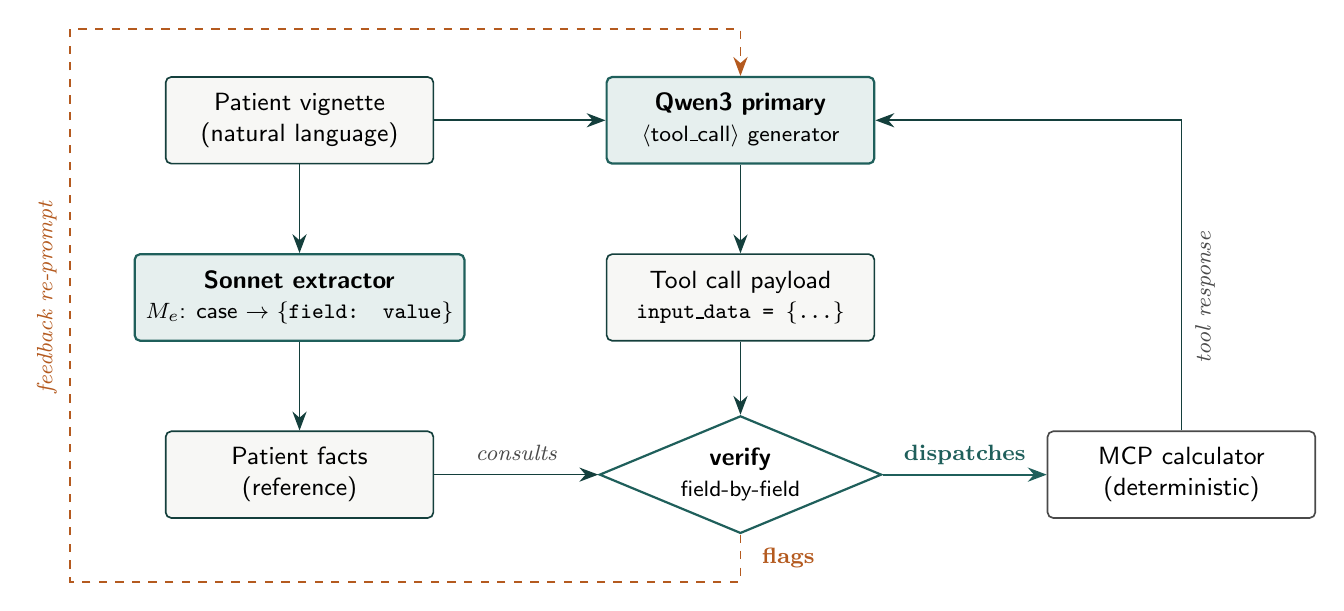
\begin{tikzpicture}[
  font=\sffamily\small,
  >={Stealth[length=2.4mm]},
  every node/.style={align=center},
  box/.style={rectangle, rounded corners=2pt, draw=accentDark, line width=0.6pt,
              minimum height=11mm, minimum width=34mm, inner sep=4pt,
              fill=paleGray},
  modelbox/.style={box, fill=accentLight, draw=accent, line width=0.8pt},
  decisionbox/.style={diamond, draw=accent, line width=0.8pt, fill=white,
                      inner sep=2pt, aspect=2.4, minimum width=30mm,
                      minimum height=14mm},
  toolbox/.style={box, fill=white, draw=warmGray},
  arrow/.style={->, draw=accentDark, line width=0.6pt},
  feedback/.style={->, draw=condBprimeE, line width=0.7pt, dashed},
  cleanpath/.style={->, draw=condReactive, line width=0.7pt},
  ret/.style={->, draw=accentDark, line width=0.6pt},
]

% ── Grid coordinates ───────────────────────────────────────────────
\def\colL{0}        % left column x
\def\colM{5.6}      % middle column x
\def\colR{11.2}     % right column x
\def\rowT{4.5}      % top row y
\def\rowC{2.25}     % middle row y
\def\rowB{0}        % bottom row y

% Clearances for the feedback wrap-around halo.
% Three independent knobs so you can tune each side without affecting
% the others. Increase a value to push that side further from the
% diagram; decrease to bring it closer.
\def\padBelow{0.6}   % gap below verify before the path turns left
\def\padLeft{1.2}    % gap left of the leftmost column (this is the LEFT channel)
\def\padAbove{0.6}   % gap above primary before the path turns right and down

% ── Nodes ──────────────────────────────────────────────────────────
\node[box]      (case)      at (\colL,\rowT) {Patient vignette\\(natural language)};
\node[modelbox] (extractor) at (\colL,\rowC) {\textbf{Sonnet extractor}\\\footnotesize $M_e$: case $\to$ \texttt{\{field: value\}}};
\node[box]      (facts)     at (\colL,\rowB) {Patient facts\\(reference)};

\node[modelbox]    (primary) at (\colM,\rowT) {\textbf{Qwen3 primary}\\\footnotesize $\langle$tool\_call$\rangle$ generator};
\node[box]         (call)    at (\colM,\rowC) {Tool call payload\\\footnotesize\texttt{input\_data = \{...\}}};
\node[decisionbox] (verify)  at (\colM,\rowB) {\textbf{verify}\\\footnotesize field-by-field};

\node[toolbox] (mcp) at (\colR,\rowB) {MCP calculator\\(deterministic)};

% ── Main flow (all straight) ───────────────────────────────────────
\draw[arrow] (case)      -- (extractor);
\draw[arrow] (extractor) -- (facts);
\draw[arrow] (case)      -- (primary);
\draw[arrow] (primary)   -- (call);
\draw[arrow] (call)      -- (verify);
\draw[arrow] (facts)     -- node[above, font=\footnotesize\itshape,
                                  text=warmGray, yshift=0.5mm]
                            {consults} (verify);
\draw[cleanpath] (verify) -- node[above, font=\footnotesize\bfseries,
                                    text=condReactive] {dispatches}
                              (mcp);

% ── Tool response: ONE right angle via |- operator ─────────────────
% (mcp.north) |- (primary.east) automatically produces:
%   1. Vertical segment UP from mcp.north to primary.east.y
%   2. Right angle at the corner
%   3. Horizontal segment LEFT to primary.east
% No diagonals are possible because |- guarantees axis-aligned paths.
\draw[ret] (mcp.north) |- (primary.east);
% Label: anchored at center on the right vertical lane.
\node[font=\footnotesize\itshape, text=warmGray,
      anchor=center, rotate=90]
  at (\colR+0.30, \rowC) {tool response};

% ── Feedback wrap (left side, balanced halo with uniform \pad) ─────
% Path corners (all axis-aligned):
%   verify.south  → (verify.south.x, verify.south.y - \pad)   [DOWN]
%                 → (colL - boxhalf - \pad, same y)             [LEFT]
%                 → (same x, primary.north.y + \pad)            [UP]
%                 → (primary.north.x, same y)                   [RIGHT]
%                 → primary.north                              [DOWN]
\coordinate (verifyBelow) at ($(verify.south)+(0,-\padBelow)$);
\coordinate (leftLane)    at ($(case.west)+(-\padLeft,0)$);
\coordinate (topLane)     at ($(primary.north)+(0,\padAbove)$);

\draw[feedback]
  (verify.south)
    -- (verifyBelow)                           % DOWN
    -- (leftLane |- verifyBelow)               % LEFT to the left lane
    -- (leftLane |- topLane)                   % UP along the left lane
    -- (primary.north |- topLane)              % RIGHT to above primary
    -- (primary.north);                        % DOWN into primary.north

% Labels positioned along the path:
%   "flags" — short action label at the start of the dashed line
%             (just to the right of where it leaves verify.south).
%   "feedback re-prompt" — descriptive label on the left vertical lane,
%             mirror-image of "tool response" on the right lane.
\node[font=\footnotesize\bfseries, text=condBprimeE,
      anchor=west]
  at ($(verify.south)+(0.15,-0.3)$) {flags};
\node[font=\footnotesize\itshape, text=condBprimeE,
      anchor=center, rotate=90]
  at ($(leftLane)+(-0.30,-2.25)$) {feedback re-prompt};

\end{tikzpicture}
\caption{Apparatus overview. Right: a clean tool call is dispatched to
MCP. Dashed left: a verifier flag re-prompts the primary.}
\label{fig:mechanism}
\end{figure}


On flag, the verifier injects the query-style intervention template
(\cref{app:feedback_template}) into the model's prompt --- naming
the disagreeing fields, the value the model proposed, and the value
the extractor found --- and re-prompts. The MCP call is \emph{not}
dispatched. On clean, the call is dispatched and the tool response is
injected back into the prompt; the loop continues. On malformed JSON,
the verifier requests a correction without comparison. Re-prompts
per vignette are capped at the value in \cref{tab:prereg_params}.

Three properties of this design are critical. First, the verifier is
\emph{blind} to whether the extractor was right --- it only knows
whether the model and the extractor disagree on a required field both
populated; the extractor's value is treated as the reference by
construction. Second, the verifier's ``no value $\rightarrow$ no
flag'' rule conservatively suppresses false positives when the
extractor abstains. Third, the schema gate guarantees that flags on
fields the calculator's output does not depend on cannot occur, so
the verifier's harm cannot be attributed to spurious flags on
inactive fields.

\subsection{The Fact Extractor}
\label{sec:methods_extractor}

The extractor's vocabulary is generated deterministically from the
MCP per-calculator JSON Schemas via the schema dump. Because both
the extractor and the verifier consume the same schemas, the
verifier \emph{cannot ask about a field the extractor cannot in
principle emit}, and the extractor cannot emit a field the MCP
backend does not recognize. This vocabulary alignment is a
structural property of the design, not a runtime invariant we have
to police.

Four extractor pipelines are evaluated. All four share the same
prompt header (\cref{lst:prompt_extractor_header}), abstention rule,
and sampling temperature ($0.7$). They differ on three orthogonal
axes:

\begin{itemize}\setlength\itemsep{2pt}
  \item \textbf{Placement.} Where extraction happens relative to tool
        calls: upfront (full-schema, once per vignette) or reactive
        (scoped to the active calculator, once per tool call).
  \item \textbf{Output format.} Whether each extracted field is a
        bare value or a \texttt{(value, source\_span)} pair anchored
        in the vignette text.
  \item \textbf{Sampling.} Whether each field's value comes from a
        single sample ($k=1$) or a majority vote over $k=3$
        independent samples.
\end{itemize}

Each primary study condition is a single point in this space:

\begin{itemize}\setlength\itemsep{2pt}
  \item B$'$+E (upfront): upfront full-schema, bare values, $k=1$.
  \item B$'$+E (reactive): reactive scoped, bare values, $k=1$.
  \item B$'$+E (reactive + citations): reactive scoped, citation pairs, $k=1$.
  \item B$'$+E (reactive + k-shot): reactive scoped, bare values, $k=3$ vote.
\end{itemize}

The mechanism arms (citations, k-shot) anchor on reactive rather
than upfront for two reasons. First, $k=3$ over a $\sim$50K-token
upfront prompt is not a credible deployment configuration. Second,
each pairwise contrast against the reactive baseline isolates a
single axis change (\cref{sec:methods_stats}), preserving
orthogonality.

\subsubsection{Upfront Pipeline}
\label{sec:methods_extractor_upfront}

One Sonnet call per vignette, at run start, covering the full
$\sim$500-field union schema. The result is fixed for the duration of
the vignette and consulted on every tool-call interception. Across
all $\sim$70 calculators in MedAI MCP, the union of property names
exceeds 500 unique fields; the schema for any single calculator
typically declares 3--30. One representative calculator's JSON
Schema is reproduced verbatim in \cref{app:bmi_schema}.

\subsubsection{Reactive Pipeline}
\label{sec:methods_extractor_reactive}

One focused Sonnet call per
\toolname{medical\_calculator\_output} tool call. At each such call,
the adapter parses the keys of the model's proposed
\verb|input_data|, builds a focused Sonnet prompt restricted to those
fields, and runs extraction blind to the model's proposed values
(the extractor sees field \emph{names} and the case text, never the
values the model proposed). The result mutates the monitor's facts
for the duration of that tool call's verification. Per-vignette
cost scales with the number of \verb|_output| calls; each call is
small (typically 3--30 fields).

\subsubsection{Reactive + Citations Pipeline}
\label{sec:methods_extractor_citations}

Identical to the reactive pipeline, except each populated field is
returned as \texttt{\{value, source\_span\}} where
\texttt{source\_span} is a verbatim substring of the vignette text.
A post-extraction validator confirms the substring property; if
validation fails, the field is treated as null (abstention).
Validation rejects paraphrase, normalization, and reformatting; only
byte-identical spans are accepted. The verifier consults the
\texttt{value} field for comparison but logs both for analysis.

\subsubsection{Reactive + k-Shot Pipeline}
\label{sec:methods_extractor_kshot}

Identical to the reactive pipeline, except each focused Sonnet call
is dispatched $k=3$ times with three independent seeds and identical
prompt at temperature $0.7$. Samples are reduced per field by
majority vote: a value present in $\ge 2$ of $3$ samples wins;
three-way disagreement yields null (abstention). The three samples
are dispatched sequentially, so the per-call extraction latency of
this pipeline is approximately $3\times$ that of the single-sample
reactive pipeline; the cost--latency reporting
(\cref{sec:results_cost}) reflects this.

The only architectural differences across the four pipelines are
\emph{when} extraction happens, \emph{what} the extractor returns,
and \emph{how many independent samples} are taken. The verifier, the
monitor, the MCP transport, the loop driver, and the response schema
are byte-identical across all four.

\subsection{Pre-Registered Statistical Analysis}
\label{sec:methods_stats}

The primary contrast family targets the experimental factor
(extractor architecture). Six paired comparisons are pre-registered;
each isolates a single design axis:

\begin{enumerate}\setlength\itemsep{2pt}
  \item B vs A --- does tool access help?
  \item B$'$ vs B --- does forced tool use help, without verifier?
  \item B$'$+E (upfront) vs B$'$ --- does upfront verifier-guided
        extraction help over forced-tool baseline?
  \item B$'$+E (reactive) vs B$'$ --- does reactive verifier-guided
        extraction help over forced-tool baseline?
  \item B$'$+E (reactive + citations) vs B$'$+E (reactive) --- does
        citation grounding improve the reactive pipeline?
  \item B$'$+E (reactive + k-shot) vs B$'$+E (reactive) --- does
        $k$-shot voting improve the reactive pipeline?
\end{enumerate}

With family $\alpha = 0.05$ and Bonferroni correction over $n = 6$
tests, the per-test threshold is $\alpha = 0.00833$. The outcome is
paired binary correctness per vignette; the test is McNemar's exact
test~\citep{mcnemar1947} on the discordant pairs. Per-condition
accuracies are reported with Wilson~\citep{wilson1927} 95\%
confidence intervals. Effect sizes ($\Delta$ accuracy in percentage
points) are reported alongside $p$-values.

Four secondary contrasts are reported outside the primary family and
are not Bonferroni-corrected: (i) B$'$+E (upfront) vs B$'$+E
(reactive), isolating placement holding all other axes fixed;
(ii) C vs B$'$, testing whether prompting the model to self-check its
inputs helps over the no-check forced-tool baseline; (iii) B$'$+E
(reactive) vs C, testing whether the external extractor--verifier
beats prompt-only self-check on the matched forced-tool footing; and
(iv) D vs B$'$, the post-hoc output-check comparator on the matched
forced-tool footing. All four comparators (C, the B$'$+E arms, and D)
now sit on the same forced-tool footing as B$'$, so they can be read
as alternative verification methods against a common no-check baseline;
the legacy unforced C-vs-B and D-vs-B comparisons are superseded.

\subsection{Apparatus Gate}
\label{sec:methods_gate}

Before accepting primary results, we replicated Sonnet on Condition
B and required the resulting accuracy to fall within
$[0.789, 0.849]$ --- $\pm 3$ pp of EkaCare's published 81.9\%
reference for Claude Sonnet 4.6 with tool access on
medical\_calculator\_eval~\citep{ekacare_error_analysis}. The gate
threshold was specified in advance in the locked pre-registration
config (recorded in each result bundle's manifest, \cref{app:logging})
and is not adjustable post-hoc. Its purpose is drift
detection on the harness, dataset, prompt rendering, and MCP
transport. It is not a validation of the primary Qwen3 results ---
we assume the harness behaves identically for the primary model
conditional on the gate.


\section{Results}
% =============================================================================
% RESULTS — populated from results/analysis/* (9-condition study).
% =============================================================================

\subsection{Apparatus Gate}
\label{sec:results_gate}

Sonnet on Condition B reached $80.4\%$ accuracy ($857/1066$),
\emph{within} the pre-registered band $[78.9\%, 84.9\%]$ defined in
\cref{sec:methods_gate}. The gate \textbf{passed}
($\Delta = -1.51$ pp from the $81.9\%$ reference). The primary contrasts
below are interpretable only because this gate held.

\FloatBarrier
\subsection{Primary Comparisons (Pre-Registered)}
\label{sec:results_primary}

\Cref{tab:accuracy} reports per-condition accuracy with Wilson 95\%
confidence intervals; \cref{tab:mcnemar_primary} reports the six
pre-registered McNemar contrasts at Bonferroni $\alpha = 0.00833$.

\begin{figure}[H]
  \centering
  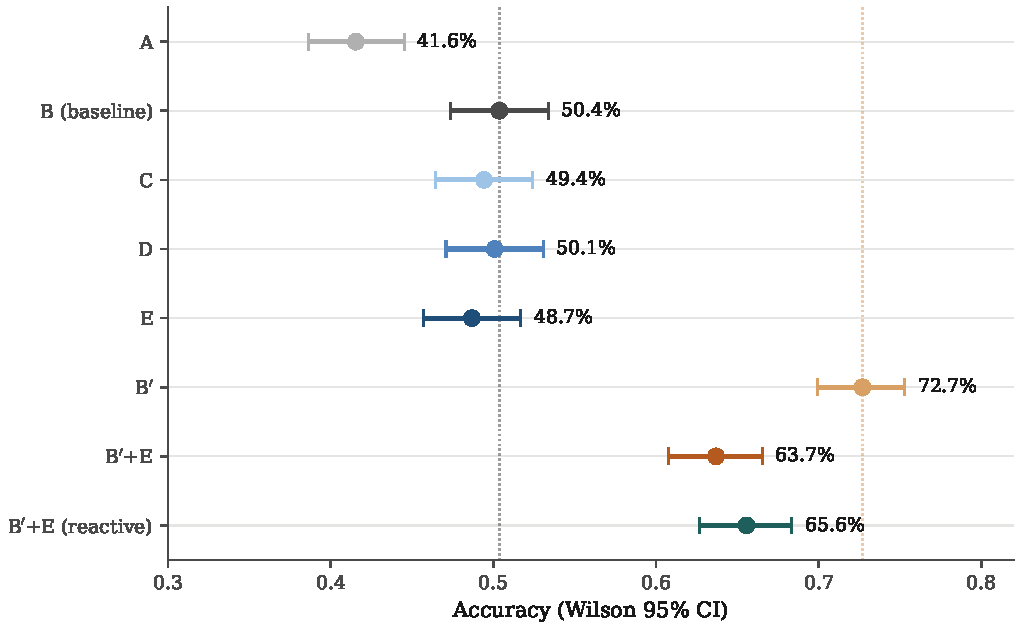
\includegraphics[width=0.92\linewidth]{forest_accuracy.pdf}
  \caption{Per-condition accuracy with Wilson 95\% confidence intervals
  ($N=1066$). Color encodes condition group.}
  \label{fig:forest}
\end{figure}

The two scaffolding contrasts behave as expected and bound the room any
verifier has to work in: tool access lifts accuracy from $41.6\%$ (A) to
$50.3\%$ (B; $\Delta = +8.7$ pp, $p_{\text{Bonf}} = 2.1\times10^{-10}$),
and forcing the model to use a calculator rather than answer from prior
knowledge lifts it further to $71.6\%$ (B$'$ vs B; $\Delta = +21.3$ pp,
$p_{\text{Bonf}} = 2.3\times10^{-36}$). Forced tool use, not the
verifier, is the dominant lever.

\textbf{No extractor pipeline improves on the forced-tool baseline.}
All four B$'$+E conditions land within $0.9$ pp of B$'$
($71.6\%$): upfront $72.5\%$, reactive $72.2\%$, reactive+citations
$72.5\%$, reactive+k-shot $72.0\%$. None of the four B$'$+E pipelines
significantly exceeds B$'$: no pre-registered contrast clears the
Bonferroni threshold (all $p_{\text{Bonf}} = 1.0$; smallest raw
$p = 0.19$, upfront vs B$'$), and the $k$-shot arm is numerically below
the reactive baseline. At
best-practice configuration the verifier shows no significant effect in
either direction; it sits on top of B$'$.

\textit{What this does and does not show.} This is a null result for
H1--H4: under schema-gating, query-style intervention, and abstention,
none of the tested extractor pipelines moved accuracy above B$'$ at the
pre-registered significance level. It does \emph{not} show that
verifier-guided extraction ``cannot help'' in principle --- the pilot
diagnostics (\cref{sec:methods_pilots}) show the same mechanism
\emph{harming} accuracy when un-gated, so best-practice hygiene's
contribution here is to remove that harm and return the verifier to
parity with B$'$, not to add value on top of it. The result is also
bounded in sensitivity: with the observed discordance ($40$--$60$
discordant pairs per B$'$+E-vs-B$'$ contrast), the $95\%$ CI on each
accuracy difference has half-width $\approx 1.3$ pp, so the design
rules out an improvement larger than $\sim$2--3 pp but is underpowered
to detect a gain of $1$--$2$ pp.

\FloatBarrier
\subsection{Extractor Architecture: Placement, Output Format, Sampling}
\label{sec:results_architecture}

This subsection reports the within-architecture contrasts among the
four primary study conditions. Each pairwise comparison isolates a
single axis (\cref{sec:methods_extractor}).

None of the three axes carries an effect; all three contrasts are far
from significance.

\textbf{Placement (upfront vs reactive).} Upfront ($72.5\%$) and
reactive ($72.2\%$) are statistically indistinguishable
($\Delta = +0.3$ pp; $30$ vs $27$ discordant; $p = 0.79$). Placement
does not change accuracy --- but it changes cost sharply
(\cref{sec:results_cost}).

\textbf{Output format (bare vs citation).} Adding verbatim source-span
grounding does not help ($72.5\%$ vs $72.2\%$; $\Delta = +0.3$ pp;
$32$ vs $29$ discordant; $p = 0.80$). Half of all citation spans were
rejected by the substring validator and coerced to null
($8{,}356/16{,}534$ accepted, $50.5\%$; \cref{sec:results_diagnostic}),
so citation grounding mostly removed fields from the comparison rather
than strengthening it.

\textbf{Sampling ($k=1$ vs $k=3$).} Majority voting does not help and is
numerically slightly worse ($72.0\%$ vs $72.2\%$; $\Delta = -0.2$ pp;
$26$ vs $28$ discordant; $p = 0.89$). The samples did diverge --- only
$61.1\%$ of field-votes showed full three-way agreement, $15.2\%$ a
$2/3$ majority, and $23.7\%$ no majority (coerced to null) --- so the
$k$-shot machinery was active, not collapsed; it simply did not improve
the reference.

\FloatBarrier
\subsection{Flag Composition}
\label{sec:results_diagnostic}

\begin{figure}[H]
  \centering
  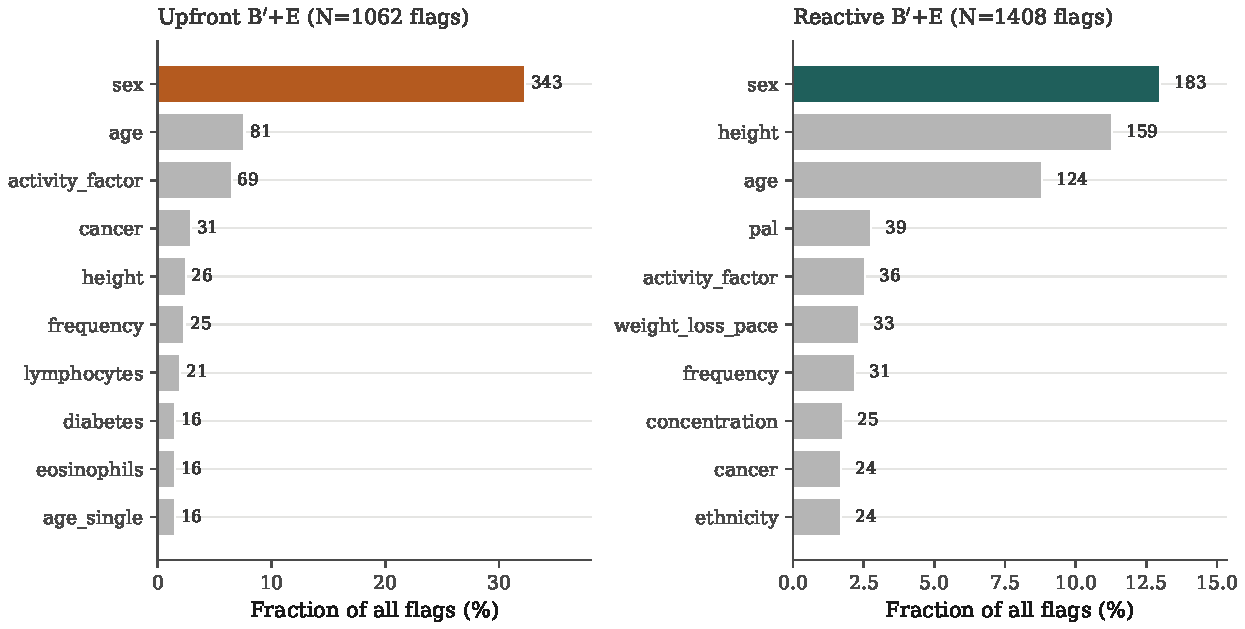
\includegraphics[width=0.98\linewidth]{flag_composition.pdf}
  \caption{Top-10 flagged fields under each primary study extractor
  pipeline.}
  \label{fig:flag_composition}
\end{figure}

Schema-gating reshapes the flag distribution as designed. Under upfront
extraction the verifier intervened on $130$ vignettes ($12.2\%$) with
$336$ total violations; by construction every flag is on a
calculator-required field, so the $58.6\%$ non-required-field share seen
in the un-gated pilot (\cref{sec:methods_pilots}) is zero here. The
single-field dominance also eases: \texttt{sex} accounts for $76/336$
flags ($22.6\%$, down from $32\%$ in the pilot), followed by
\texttt{age} ($29$), \texttt{activity\_factor} ($19$), and
\texttt{height} ($15$). On the rows where the verifier did fire, the
model still produced the correct final answer $74.6\%$ of the time ---
i.e.\ most interventions did not rescue a wrong answer, consistent with
the null accuracy effect.

Reactive extraction fires more often ($172$ rows, $16.1\%$; $524$
violations) and its flags concentrate jointly on \texttt{height} ($73$)
and \texttt{sex} ($73$), with \texttt{age} ($53$) third; its
correct-on-intervention rate is lower ($66.9\%$). The reactive pipeline
re-extracts at each tool call, so common fields are re-checked more
often --- more flags, but no better accuracy.

\FloatBarrier
\subsection{Per-Category and Stratified Effects}
\label{sec:results_category}

\begin{figure}[H]
  \centering
  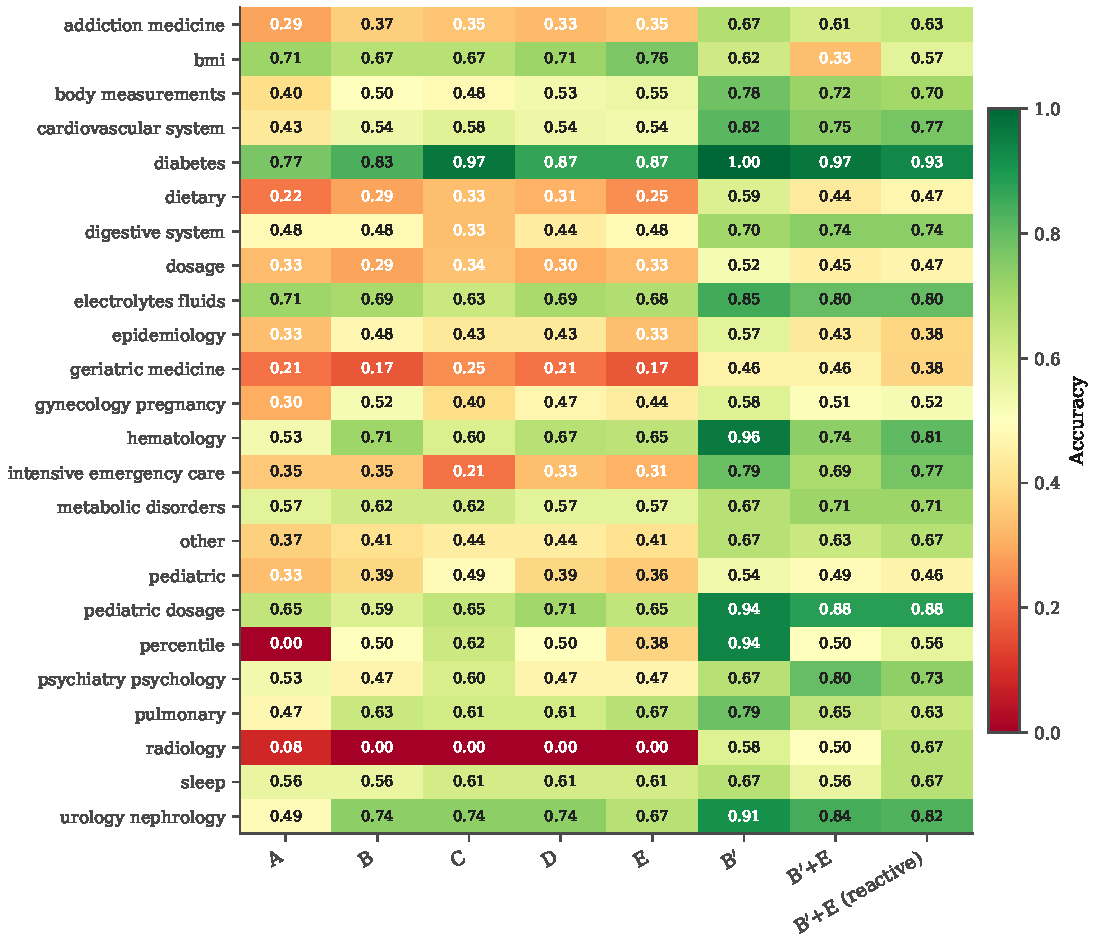
\includegraphics[width=0.92\linewidth]{category_heatmap.pdf}
  \caption{Accuracy by calculator category $\times$ condition, for the
  primary comparison: B$'$ and the four B$'$+E pipelines. (Per-category
  values for the other conditions are recomputable from the released
  per-vignette data.)}
  \label{fig:category_heatmap}
\end{figure}

No calculator category shows a systematic B$'$+E gain over B$'$. Across
the 24 categories the per-condition differences are small and
non-monotonic --- upfront edges B$'$ in a few low-$n$ categories (e.g.\
BMI $0.52\to0.62$, percentile $0.81\to0.94$, hematology $0.89\to0.94$)
but is level or behind in others (e.g.\ cardiovascular $0.81\to0.79$,
dietary $0.60\to0.59$) --- consistent with noise around a null main
effect rather than a localized benefit.

Restricting to the $166$ vignettes on which \emph{every} condition
invoked a tool (the stratified subset) does not change the picture:
B$'$ reaches $75.3\%$ and the four B$'$+E pipelines fall between
$72.3\%$ and $75.9\%$, all overlapping. On this tool-using subset the
no-tools floor A collapses to $15.7\%$, underscoring that the headline
accuracy is carried by tool use, not by verification.

\FloatBarrier
\subsection{Cost and Latency}
\label{sec:results_cost}

\Cref{fig:pareto} plots the cost--accuracy frontier;
\cref{tab:cost} summarizes per-vignette token and latency numbers.

\begin{table}[!htbp]
  \centering
  \caption{Per-vignette tokens (from the full $N=1066$ run) and median
  single-request latency (from a fixed-concurrency timing pass at one
  worker, $N=50$). ``API'' tokens are Sonnet calls (extractor + post-hoc
  verifier in D); ``On-GPU'' tokens are Qwen3 via vLLM. Tokens are
  load-independent; latency is reported only from the fixed-concurrency
  pass because the full run uses a different worker count per condition
  (\cref{sec:methods_compute}) and its wall-clock is therefore not
  comparable across conditions.}
  \label{tab:cost}
  \begin{tabular}{lrrr}
    \toprule
    Condition & Total tokens & API tokens & Latency (s) \\
    \midrule
    A                                & $2{,}976$  & $0$       & ---    \\
    B (baseline)                     & $8{,}328$  & $0$       & $15.5$ \\
    B$'$                             & $29{,}901$ & $0$       & $47.5$ \\
    B$'$+E (upfront)                 & $78{,}836$ & $47{,}478$ & $49.9$ \\
    B$'$+E (reactive)                & $32{,}211$ & $928$     & $52.1$ \\
    B$'$+E (reactive + citations)    & $32{,}570$ & $1{,}063$ & $55.5$ \\
    B$'$+E (reactive + k-shot)       & $34{,}121$ & $2{,}823$ & $68.7$ \\
    C                                & $29{,}785$ & $0$       & $54.8$ \\
    D                                & $31{,}951$ & $971$     & $56.9$ \\
    \bottomrule
  \end{tabular}
\end{table}

The four pipelines reach the same accuracy at very different cost, so
the comparison is decided entirely on cost. Upfront extraction is the
clear outlier: its single full-schema ($\sim$500-field) Sonnet call
costs $\sim$$47$K API tokens per vignette and drives total tokens to
$78{,}836$ --- roughly $2.4\times$ the reactive pipeline's $32{,}211$
for identical accuracy ($72.5\%$ vs $72.2\%$). The two mechanism arms
add cost without accuracy: citations is essentially free over reactive
($+359$ tokens) but $k$-shot triples the extractor's API tokens
($928 \to 2{,}823$) and is the slowest pipeline at $68.7$ s median
single-request latency, because its three samples dispatch
sequentially. Reactive is therefore Pareto-dominant among the verifier
pipelines --- cheapest in tokens, second-fastest, and tied on accuracy.
None of them, however, is Pareto-efficient against B$'$ itself
($29{,}901$ tokens, $47.5$ s), which matches their accuracy at lower
cost.

\begin{figure}[H]
  \centering
  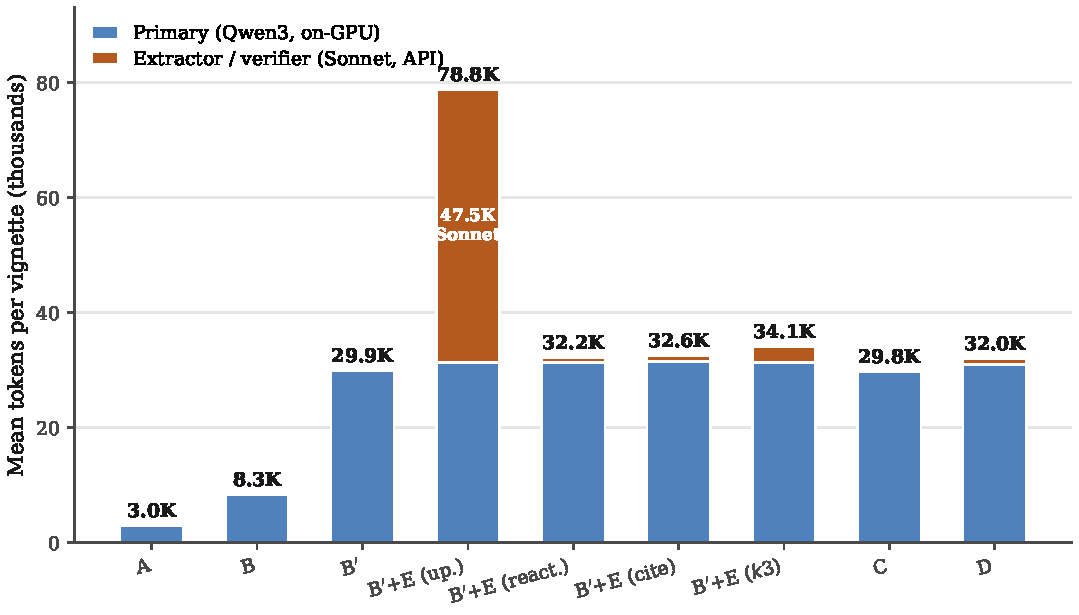
\includegraphics[width=0.92\linewidth]{token_decomposition.pdf}
  \caption{Per-vignette token cost decomposed into primary-model and
  external API tokens.}
  \label{fig:tokens}
\end{figure}

\begin{figure}[H]
  \centering
  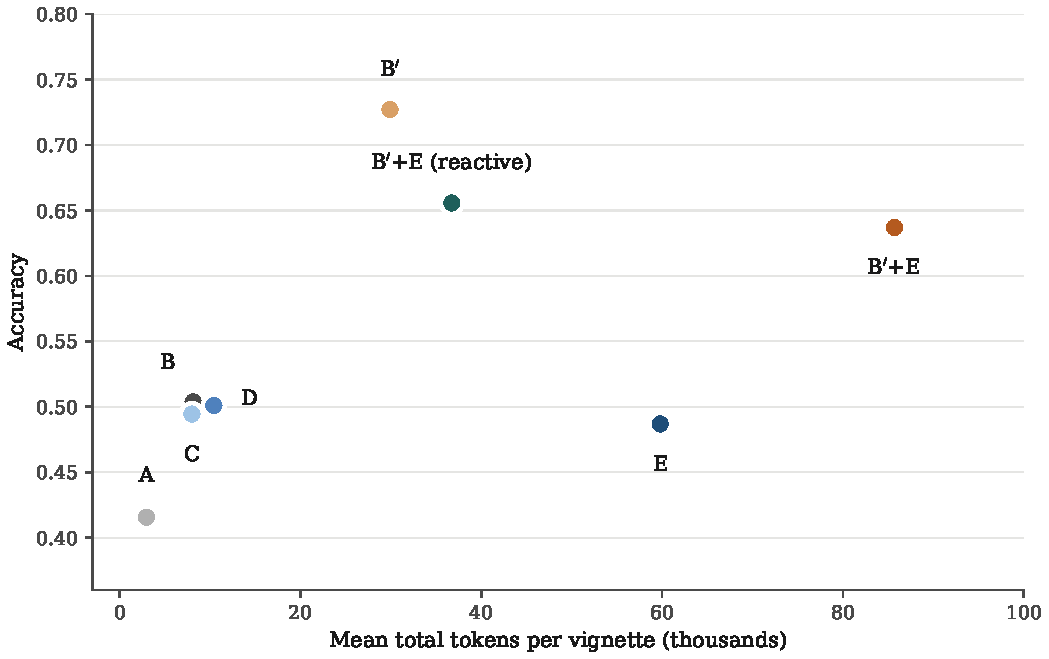
\includegraphics[width=0.88\linewidth]{pareto.pdf}
  \caption{Cost--accuracy frontier.}
  \label{fig:pareto}
\end{figure}

\begin{figure}[H]
  \centering
  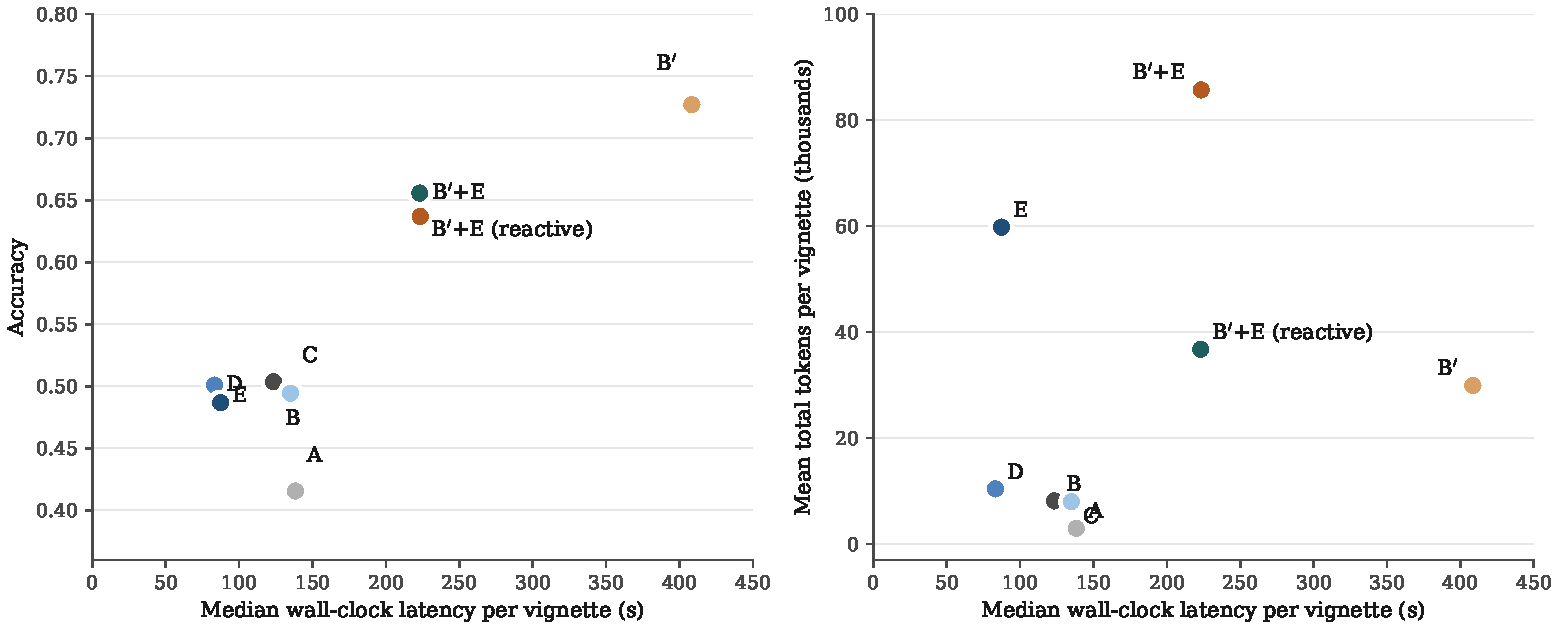
\includegraphics[width=\linewidth]{latency_panels.pdf}
  \caption{Latency vs accuracy (left) and latency vs token cost
  (right).}
  \label{fig:latency}
\end{figure}

% ─── Tables ───────────────────────────────────────────────────────────────
\begin{table}[!htbp]
  \centering
  \caption{Per-condition accuracy with Wilson 95\% CIs ($N=1066$).
  Primary-family contrasts marked with $\dagger$ are
  Bonferroni-corrected at family $\alpha=0.05$.}
  \label{tab:accuracy}
  \begin{tabular}{lccc}
    \toprule
    Condition & Group & Accuracy & 95\% CI \\
    \midrule
    A                                & anchor       & $41.6\%$ & $[38.6, 44.5]$ \\
    B (baseline)                     & anchor       & $50.3\%$ & $[47.3, 53.3]$ \\
    B$'$                             & anchor       & $71.6\%$ & $[68.8, 74.2]$ \\
    B$'$+E (upfront)$^\dagger$        & primary      & $72.5\%$ & $[69.8, 75.1]$ \\
    B$'$+E (reactive)$^\dagger$       & primary      & $72.2\%$ & $[69.5, 74.8]$ \\
    B$'$+E (reactive + citations)$^\dagger$ & primary & $72.5\%$ & $[69.8, 75.1]$ \\
    B$'$+E (reactive + k-shot)$^\dagger$ & primary  & $72.0\%$ & $[69.3, 74.7]$ \\
    C                                & exploratory  & $69.1\%$ & $[66.3, 71.8]$ \\
    D                                & exploratory  & $70.7\%$ & $[67.9, 73.4]$ \\
    \bottomrule
  \end{tabular}
\end{table}

\begin{table}[!htbp]
  \centering
  \caption{Pre-registered McNemar contrasts (Bonferroni
  $\alpha=0.00833$). Discordant pairs $(b, c)$: $b$ = correct in
  left condition only; $c$ = correct in right condition only.}
  \label{tab:mcnemar_primary}
  \begin{tabular}{lcccc}
    \toprule
    Comparison & $b$ & $c$ & $p_{\text{Bonferroni}}$ & Sig.? \\
    \midrule
    B vs A                                                       & $143$ & $50$ & $2.1\times10^{-10}$ & yes \\
    B$'$ vs B                                                    & $271$ & $44$ & $2.3\times10^{-36}$ & yes \\
    B$'$+E (upfront) vs B$'$                                     & $29$  & $19$ & $1.0$               & no  \\
    B$'$+E (reactive) vs B$'$                                    & $32$  & $25$ & $1.0$               & no  \\
    B$'$+E (reactive + citations) vs B$'$+E (reactive)           & $32$  & $29$ & $1.0$               & no  \\
    B$'$+E (reactive + k-shot) vs B$'$+E (reactive)              & $26$  & $28$ & $1.0$               & no  \\
    \bottomrule
  \end{tabular}
\end{table}

\begin{table}[!htbp]
  \centering
  \caption{Secondary contrasts (uncorrected). Within-architecture
  placement comparison and exploratory verifier-mechanism
  comparators.}
  \label{tab:mcnemar_exploratory}
  \begin{tabular}{lcccr}
    \toprule
    Comparison & $b$ & $c$ & $p$ & $\Delta$ acc \\
    \midrule
    B$'$+E (upfront) vs B$'$+E (reactive)   & $30$ & $27$ & $0.79$   & $+0.3$ \\
    C vs B$'$                               & $61$ & $87$ & $0.040$  & $-2.4$ \\
    B$'$+E (reactive) vs C                  & $88$ & $55$ & $0.0075$ & $+3.1$ \\
    D vs B$'$                               & $38$ & $47$ & $0.39$   & $-0.8$ \\
    \bottomrule
  \end{tabular}
\end{table}

\subsection{Dropped Vignettes and Completion}
\label{sec:results_completion}

No vignettes were dropped: all nine conditions scored the full
$N = 1066$, so no accuracy number is computed over a reduced
denominator and the pre-registered $2\%$ dropped-$N$ investigation
threshold (\cref{tab:prereg_params}) was never approached. Parse
failures --- replies from which no numeric prediction could be
extracted, scored as wrong per \cref{sec:methods_benchmark} --- are
rare and comparable across conditions: $1$ for A, $11$ for B, $20$ for
B$'$, $22$--$27$ across the four B$'$+E pipelines, $15$ for C, and $18$
for D (at most $2.5\%$ of rows). Their near-uniformity across conditions
means they do not differentially advantage any pipeline.


\section{Discussion}
% =============================================================================
% DISCUSSION — 9-condition study, populated from the result bundle.
% Findings (5.1) and the cost-model/tool-forcing interpretation (5.2-5.3)
% draw on results/analysis/*; threats (5.5) and scope (5.7) are general.
% =============================================================================

\subsection{Principal Findings}
\label{sec:disc_summary}

We restate the four pre-registered hypotheses
(\cref{sec:intro_hypothesis}) and the outcome of each, drawing only on
the contrasts in \cref{sec:results_primary,sec:results_architecture}.

\begin{itemize}\setlength\itemsep{3pt}
  \item \textbf{H1/H2 (does best-practice verifier-guided extraction
        beat B$'$?).} No. Both upfront ($72.5\%$ vs $71.6\%$;
        $p_{\text{Bonf}} = 1.0$) and reactive ($72.2\%$;
        $p_{\text{Bonf}} = 1.0$) are statistically indistinguishable
        from B$'$. Neither cleared the Bonferroni threshold; neither
        came close.
  \item \textbf{H3 (citations).} No. Citation grounding does not move
        accuracy over reactive ($+0.3$ pp, $p = 0.80$) --- and half of
        all source spans failed substring validation, so it mostly
        removed fields from the comparison.
  \item \textbf{H4 ($k$-shot).} No. $k=3$ voting is if anything
        slightly worse than single-sample reactive ($-0.2$ pp,
        $p = 0.89$), despite the samples genuinely diverging
        ($23.7\%$ of field-votes reached no majority).
  \item \textbf{Anchor (does tool access help?).} Yes, decisively, and
        this is where the accuracy lives: tool access (B vs A,
        $+8.7$ pp) and especially forced tool use (B$'$ vs B,
        $+21.3$ pp) are the only significant primary contrasts. They
        bound the room a verifier has to improve and are not themselves
        claims about verification.
\end{itemize}

The four primary hypotheses therefore all fail to reject the null: at
best-practice configuration the input verifier sits on top of B$'$
without moving accuracy. The rest of this section explains \emph{why}
the gap is null --- and why that is the expected outcome once the
reference layer is taken seriously.

\subsection{Interpreting a Residual Gap: The Reference Layer}
\label{sec:disc_extractor}

The verifier in this study is deterministic
(\cref{sec:methods_verifier}): exact match on enums, numeric tolerance
on numbers, canonical-form match on booleans, and no flag at all when
the extractor abstains. None of that machinery can synthesize a wrong
flag on its own --- a spurious flag requires a wrong reference, and the
reference comes from the LLM extractor. The extracted reference is
therefore the load-bearing component, and any gap between a
best-practice extractor pipeline and B$'$ localizes there rather than
in the comparison logic.

We state the limit as a cost model. Where the verifier's reference is
produced by an extractor $M_e$ over a required-field set $\mathcal{F}$,
the verifier's net effect on accuracy is governed by the joint
distribution of three terms:
(a) the primary model's input-error rate on $\mathcal{F}$ --- the
errors a true flag can fix;
(b) $M_e$'s extraction-error rate on $\mathcal{F}$ --- the errors that
produce false flags;
(c) the asymmetric cost of a false flag (which re-prompts and can flip
a correct call to wrong) versus a true flag (which can fix a wrong
call).
Verification helps only when true flags outweigh false flags under
this cost. The schema gate (\cref{sec:methods_verifier}) restricts the
comparison to required fields, which shrinks the surface on which term
(b) can act; the four extractor pipelines vary placement, output
format, and sampling, each of which is a different attempt to lower
term (b). Empirically, none of the three levers moved accuracy, so none
measurably shifted the balance of terms (a)--(c). The flag statistics
are consistent with this: reactive extraction fired \emph{more} often
than upfront ($16.1\%$ vs $12.2\%$ of vignettes) yet had a \emph{lower}
correct-on-intervention rate ($66.9\%$ vs $74.6\%$), so its extra
interventions were not net-corrective. The likeliest reading is that,
once tool use is forced, the primary model's input-error rate on
required fields (term a) is already low --- B$'$ alone reaches
$71.6\%$ --- so there are few wrong calls for a true flag to rescue,
while the residual false flags from term (b) roughly cancel whatever
true flags remain. The verifier lands at parity because, post-gating,
both kinds of flag are rare and approximately balanced.

A subtlety the cost model alone misses: ``extraction error'' is
broader than ``the extractor read the wrong value.'' A flag can fire
when the extractor's value is semantically correct but serialized
differently from the model's (the \texttt{sex=female} vs
\texttt{sex=1} pattern traced in \cref{app:loop_trace}). The binding
constraint there is the join of (extractor canonical form, verifier
comparison strictness, model serialization) --- any one of the three
can drive a flag the other two cannot resolve. This residue persists
under schema-gating: \texttt{sex} is still the most-flagged field
($22.6\%$ of upfront flags, co-top under reactive) --- the same field
that drives the \texttt{bmi\_001} trace, where the extractor's
semantically-correct \texttt{female} and the model's \texttt{1} disagree
only in encoding. Schema-gating removed flags on fields the calculator
ignores, but it cannot reconcile encoding mismatches on \emph{required}
fields, so this join keeps term (b)'s false-flag floor above zero and
is one concrete reason the verifier cannot get ahead of B$'$.

\subsection{Why Tool-Forcing Amplifies the Reference}
\label{sec:disc_toolforcing}

The verifier fires once per tool call, so its leverage scales with the
tool-call rate. The B$'$ prompt forces a tool call on every vignette
and removes the model's option to decline when uncertain; on every
such call the verifier injects feedback carrying the extracted
reference. This amplifies whatever the reference does: a reliable
reference is applied more often (more fixes), and an unreliable one is
applied more often (more mis-corrections). The amplification is
multiplicative in the tool-call rate, and its sign is set entirely by
the reference quality of \cref{sec:disc_extractor} --- forcing is not
harmful or helpful on its own. Here the amplification ran to a wash:
forcing raised the verifier's exposure as designed (the model emits
$\sim$$3.7$ tool calls per vignette and the verifier intervened on
$12.2\%$--$16.1\%$ of vignettes), but with post-gating flags roughly
balanced between true and false, the larger exposure moved net accuracy
in neither direction. This is the benign face of the \emph{same}
amplification that, un-gated, produced the pilot's $\sim$$9$ pp harm
(\cref{sec:methods_pilots}): schema-gating shrank the false-flag surface
enough that forcing no longer multiplies a net-negative signal.

\subsection{Implications for Deploying Verifier-Guided Reasoning in Clinical AI}
\label{sec:disc_implications}

Two recommendations follow from the mechanism regardless of the
headline numbers; a third is conditional on them.

\textit{Validate the reference pipeline independently before adopting
intermediate verification.} The verifier's correctness guarantee is no
stronger than the extractor's field-level accuracy on the deployment's
live field distribution. A held-out, hand-annotated field-accuracy
gate on the fields the deployment actually uses --- not the union of
all possible MCP fields --- is the precondition the cost model in
\cref{sec:disc_extractor} implies.

\textit{Prefer a non-LLM reference where one exists.} Where structured
patient data are available (EHR fields, device vitals, LIS results),
they remove term (b) for the fields they carry. Reserve LLM extraction
for fields the structured record does not hold.

\textit{Choose the extractor pipeline on the measured cost--accuracy
frontier.} Among the verifier pipelines, reactive extraction dominates:
it matches upfront's accuracy at $\sim$$40\%$ of the token cost
($32$K vs $79$K per vignette) and is faster than $k$-shot
(\cref{sec:results_cost}). But on this benchmark \emph{no} pipeline is
Pareto-efficient against B$'$ itself, which matches their accuracy at
lower cost --- so input verification earns its overhead only where the
reference can be made more reliable than a single best-practice LLM
extractor, i.e., under the first two recommendations above.

\subsection{Threats to Validity}
\label{sec:disc_limitations}

\textit{Single primary model.} All conditions evaluate
Qwen3-30B-A3B-Thinking-2507. The mechanism we identify (the extracted
reference as the binding component) should transfer across models, but
the magnitudes will not.

\textit{Single benchmark.} medical\_calculator\_eval covers
deterministic calculator dispatch with typed inputs. Generalization to
differential-diagnosis, triage, or open-ended tool surfaces --- where
inputs are less structured --- is untested.

\textit{Single extractor model.} Sonnet 4.6 is one extractor; another
could show different per-field error rates and thus a different verdict.
The claim is that \emph{some} LLM extractor is the binding constraint,
not that Sonnet specifically fails.

\textit{No ground-truth-reference comparator.} No condition consults a
hand-annotated reference, which would isolate the verifier mechanism
from extractor fallibility entirely. This is the most important
comparator the study lacks (\cref{sec:disc_followups}).

\textit{Conservative verifier is silent on extractor misses.} The ``no
extractor value $\rightarrow$ no flag'' rule (\cref{sec:methods_verifier})
suppresses false positives but makes a silent extractor (one that
extracts nothing for a field the model proposes) invisible to the
firing-rate statistics. Some fraction of vignettes may carry silent
verifier failures the firing counts cannot see.

\textit{Extractor stochasticity.} The extractor runs at temperature
$0.7$ (and $k=3$ in one pipeline), so its reference is not
deterministic across runs. The $k$-shot diagnostics quantify the
variance directly: across $20{,}271$ field-votes, $61.1\%$ showed full
three-way agreement, $15.2\%$ a $2/3$ majority, and $23.7\%$ no majority
at all. So the reference does vary across samples on a meaningful
minority of fields --- but that variance falls on ambiguous fields,
not on the common ones (\texttt{sex}, \texttt{age}, \texttt{height})
that dominate both the flag counts and the accuracy-relevant decisions.
A repeated run would shift total flag counts slightly without changing
the architectural pattern or the null verdict.

\textit{Apparatus-gate scope.} The gate (\cref{sec:methods_gate})
detects drift on the harness, dataset, prompt rendering, and MCP
transport via Sonnet on Condition B. It does not independently validate
the primary Qwen3 numbers; we assume the harness behaves identically
for the primary model conditional on the gate holding.

\subsection{Future Directions}
\label{sec:disc_followups}

The study fixes the verifier and varies only the extractor pipeline.
Three reference-layer variants are the natural next experiments, each
holding all other variables at this study's values. We list them as
hypothesized future work, not as findings.

\begin{itemize}\setlength\itemsep{2pt}
  \item \textbf{Hand-annotated ground-truth reference.} Removes the LLM
        extractor entirely and answers whether procedural input
        verification helps when the reference is reliable. Cost:
        annotation of all $1{,}066$ vignettes.
  \item \textbf{Multi-LLM ensemble extractor.} Requires agreement
        across $\ge 2$ extractor models before the verifier's reference
        is populated, targeting single-model variance in term (b).
  \item \textbf{Structured-record reference.} A non-LLM reference layer
        (e.g., EHR-keyed inputs) for a deployment-realistic setting;
        requires a benchmark that ships structured records alongside
        vignettes, which medical\_calculator\_eval does not.
\end{itemize}

\subsection{What This Paper Does Not Claim}
\label{sec:disc_notclaim}

To preempt common misreadings, we name the claims this paper does
\emph{not} make.

\textbf{1. ``Interwhen does not work.''} Interwhen's verify/fix
mechanism operates as designed in every condition we run. Our
adaptation repurposes its LLM extraction step to recover an independent
reference from the case rather than the model's asserted state from the
trace (\cref{sec:bg_interwhen}); any limit we find is in that reference
layer, not the mechanism.

\textbf{2. ``Output verification is unhelpful.''} We study procedural
\emph{input} verification specifically (\cref{sec:bg_surfaces}). Output
verification, outcome verification, grounded retrieval, and
human-in-the-loop regimes are different surfaces; Condition D is the
only output-style comparator here and is scoped as a control, not the
object of study.

\textbf{3. ``Sonnet is a poor extractor.''} Sonnet 4.6 is near the
frontier of clinical-text extraction. Any underperformance we attribute
to the extractor is a property of the prompt regime (e.g., a
$\sim$500-field upfront schema), not the model's underlying capability.

\textbf{4. ``Tool-forcing prompts are dangerous.''} Forcing amplifies
whatever follows it in both directions (\cref{sec:disc_toolforcing}).
With a reliable reference the amplification is beneficial; the prompt
is not harmful on its own.

\textbf{5. ``Any one pipeline is the right deployment configuration.''}
Each contrast is one mechanistic test. A production choice depends on
the measured cost--latency frontier, field-level validation of the
extractor, and the specific clinical workflow --- more than a single
accuracy contrast can settle.


\section{Conclusion}
% =============================================================================
% CONCLUSION
% =============================================================================

We evaluated interwhen-style procedural input verification on a
clinical tool-calling benchmark across nine conditions spanning three
groups: capability anchors (A, B, B$'$), a primary study of four
extractor pipelines under best-practice configuration (upfront,
reactive, reactive + citations, reactive + k-shot), and two
exploratory verifier-mechanism comparators (C, D). Six paired
contrasts were pre-registered at family $\alpha=0.05$.

Best-practice verifier-guided extraction did not move accuracy above
B$'$. All four extractor pipelines matched the forced-tool baseline
($71.6$--$72.5\%$) with no significant contrast, and no architectural
axis --- placement, citation grounding, or $k$-shot voting --- carried
an effect. System accuracy is set by forced tool use ($+21.3$ pp over
plain tool access); the input verifier, at best-practice configuration,
neither helps nor hurts. Among the pipelines, reactive extraction is
the deployment choice --- identical accuracy at $\sim$$40\%$ of
upfront's token cost. The exploratory alternatives are consistent:
prompting the model to self-check (C) is no better than B$'$, post-hoc
output review (D) is no better than B$'$, and the external verifier
beats prompt-only self-check head-to-head.

Two design choices in the primary study --- the schema-gated verifier
and the query-style intervention --- were motivated by pilot
diagnostics (\cref{sec:methods_pilots}) and address by construction two
failure modes those pilots exposed. That gap proves to be null:
best-practice hygiene removes the harm the un-gated pilot caused but
produces no benefit over the forced-tool baseline, locating the binding
constraint in the LLM-extracted reference rather than the verifier
mechanism itself.


\section*{Code and Data Availability}
The full experimental harness --- including the orchestration notebook,
per-condition adapter code, the deterministic input verifier, the schema-aligned
fact extractor, and the analysis pipeline --- is available at
\url{https://github.com/jackyang25/interwhen-karma-harness}.
The \toolname{medical\_calculator\_eval} benchmark is distributed by
EkaCare via the KARMA framework; we use the public release without
modification.

The complete per-condition result bundle (raw model outputs, scored rows,
McNemar contingency tables, manifests with SHA-256 checksums, the MCP
calculator schema dump used at runtime, and the regenerated extractor
prompt) is committed to the same repository under \texttt{results/},
indexed by a manifest JSON that lists every artifact with its SHA-256
checksum. Schema dumps are included in each bundle's provenance
subdirectory so the extractor prompt can be regenerated byte-identically
from the source schemas.

All runs are deterministic by construction: model temperature is zero,
the schema dump is frozen at run start, and the extractor prompt is
generated deterministically from the dump. Re-running the harness on the
same benchmark with the same seeds and the same MCP schema dump
reproduces the per-vignette outcomes used in this paper.


\section*{Funding and Conflicts of Interest}
% [USER INPUT NEEDED] Funding and affiliation details removed for
% anonymous review. Restore institutional wording for the camera-ready
% version.
Funding information has been removed for anonymous review. The authors
declare no competing financial or non-financial interests related to
this work.


\section*{Acknowledgments}
The authors thank the interwhen team at Microsoft Research India for
discussions of the verifier-guided reasoning framework this work adapts,
and for making the reference implementation available. We thank the
EkaCare team for releasing the \toolname{medical\_calculator\_eval}
benchmark and the MedAI MCP toolset that made this study possible. The
Qwen team is acknowledged for the public release of
Qwen3-30B-A3B-Thinking-2507, and Anthropic for the Sonnet 4.6 model
used as the fact extractor.

% [USER INPUT NEEDED] Optionally add specific reviewers or named
% collaborators here once their consent is confirmed.


\bibliographystyle{abbrvnat}
\bibliography{references}

\clearpage
\appendix
\section{Reference Artifacts}
% =============================================================================
% APPENDIX — Reference Artifacts
% Every prompt and schema used in the study, reproduced verbatim for
% transparency. Plus the real-data trace of one vignette.
% =============================================================================

\subsection{System Prompts}
\label{app:system_prompts}

The system prompts below differentiate conditions B$'$, C, and D. Conditions
A, B, and E use no system prompt (the dataset's per-row
\emph{confinement instruction}, described in \cref{sec:methods_benchmark},
is the only prompt suffix appended).

\begin{lstlisting}[caption={Condition B$'$ --- force tool use. Verbatim
from \toolname{prompts/condition\_b\_prime.txt}.},
label={lst:prompt_bprime}, language=]
You are an expert clinician answering medical calculator questions for
Indian patients.

You must call the appropriate calculator tool for every computation — do
not compute values by hand, even if you believe the answer is obvious.
Always invoke the matching `medical_calculator_*` tool with inputs taken
directly from the patient case, and use the tool's returned value as
your answer.

Read the case carefully, and after the tool returns, reply strictly
with the JSON object the user requests.
\end{lstlisting}

\begin{lstlisting}[caption={Condition C --- prompt-only self-verify.
Verbatim from \toolname{prompts/condition\_c.txt}.},
label={lst:prompt_c}, language=]
You are an expert clinician answering medical calculator questions for
Indian patients.

Before calling any calculator tool, verify each input you plan to pass
against the patient case: confirm the units match (e.g. mg/dL vs
mmol/L), the enum choices are correct (e.g. sex, activity level,
severity), and the numeric values are taken directly from the vignette.
If the case lacks clear evidence for a required input, do not guess —
re-read the case before calling the tool.

Read the case carefully, use any available tools if useful, and reply
strictly with the JSON object the user requests.
\end{lstlisting}

\begin{lstlisting}[caption={Condition D --- post-hoc Sonnet verifier
system prompt. Verbatim from \toolname{prompts/condition\_d.txt}.},
label={lst:prompt_d}, language=]
You are a verification reviewer for clinical calculator answers.

You will be shown (1) a patient case in Indian clinical language, (2)
the question's required output format, and (3) a candidate JSON answer
produced by another model. Your job is to identify whether the
candidate answer is consistent with the case — specifically, whether
the inputs the answering model used (if visible in its reasoning) match
what the case states.

Reply with a JSON object of the form:
{
  "consistent": true | false,
  "issue": "<one-sentence description of the discrepancy if
   consistent=false, otherwise empty string>"
}

Be conservative: only flag clear inconsistencies in units, enum choices
(sex, activity level, severity, etc.), or numeric values that
contradict the case. Do not flag minor formatting differences or
stylistic choices. Do not flag a missing field unless the question
requires it. If you are not certain there is an inconsistency, return
consistent=true.
\end{lstlisting}

\subsection{Fact Extractor Prompt}
\label{app:extractor_prompt}

The fact extractor used in E, B$'$+E, and B$'$+E (reactive) runs Sonnet
with the system prompt shown in \cref{lst:prompt_extractor_header},
followed by a schema body that is generated deterministically from the
MCP per-calculator JSON Schemas. For the upfront variant the body is
the full union of all calculator fields ($\sim$500 entries); for the
reactive variant it is the subset of fields the active tool call
requests (typically 3--30). The header and rules are byte-identical
across the two variants; only the schema body differs.

\begin{lstlisting}[caption={Fact extractor system prompt header
(stable across upfront and reactive variants). The schema body that
follows is generated programmatically from the MCP schema dump by
\toolname{harness/extraction/prompt\_builder.py}.},
label={lst:prompt_extractor_header}, language=]
You are a medical fact extractor. Read the patient vignette and return
a strict JSON object capturing every value the case explicitly states
for the fields below.

Return ONLY a JSON object (no prose, no markdown fences). Include ONLY
the fields the case explicitly states a value for. Omit any field the
case does not state — do not emit null for absent fields. The schema
below is the vocabulary of allowed field names; you do not need to
emit every field.

Rules:
- Include only what the case explicitly states. If a value must be
  inferred, computed, or guessed, omit the field.
- Use the units the case provides. Do not convert units. If the case
  says "creatinine 130 µmol/L", store 130, not the converted mg/dL value.
- For ranges (e.g. "BP 140/90"), split into the appropriate fields.
- For descriptors that map to a calculator's enum (e.g. "sedentary
  lifestyle" → "sedentary"), use the enum value if the mapping is
  unambiguous; otherwise omit.
- If the case uses Hinglish or non-standard phrasing, interpret in
  standard clinical context where unambiguous; otherwise omit.
- Return only valid JSON. No commentary.

Schema (allowed field names with type/range/enum constraints):
{ ...generated schema body... }
\end{lstlisting}

\subsection{Verifier Feedback Template (Condition E)}
\label{app:feedback_template}

The verifier's flag injects the following template into the primary
model's prompt. The \toolname{\{violations\}} placeholder expands to a
list of disagreeing fields, each annotated with the planned value, the
extracted value, and a short diagnostic note.

\begin{lstlisting}[caption={Verifier feedback prompt, verbatim from
\toolname{prompts/condition\_e\_feedback.txt}.},
label={lst:feedback}, language=]
Your planned tool call has an input that does not match the patient case:

{violations}

Re-read the case carefully and call the tool again with corrected
inputs. If the case truly does not specify the required input, do not
invent a value; explain in your reply.
\end{lstlisting}

\subsection{Example MCP Calculator Schema}
\label{app:bmi_schema}

Across all $\sim$70 calculators in MedAI MCP, the union of property
names exceeds 500 unique fields; the schema for any single calculator
typically declares 3--30. One representative calculator's JSON Schema
is reproduced verbatim below.

\begin{lstlisting}[caption={Abbreviated MCP JSON Schema for
\toolname{bmi\_calculator\_body\_mass\_index}. The full schema includes
descriptions, units, and range constraints for each field. Note that
\texttt{sex} is declared but \emph{not} required; the BMI calculator
will dispatch without it.}, label={lst:bmi_schema}, language=]
{
  "name": "bmi_calculator_body_mass_index",
  "input_data": {
    "type": "object",
    "required": ["height", "mass"],
    "properties": {
      "sex":     { "$ref": "#/$defs/Sex", "description": "Biological sex" },
      "height":  { "type": "number",  "description": "Height in meters" },
      "mass":    { "type": "number",  "description": "Body weight in kilograms" },
      "age":     { "type": "integer", "description": "Age in years" },
      "athlete": { "$ref": "#/$defs/YesNo", "description": "Athletic status" }
    }
  }
}
\end{lstlisting}

\subsection{Real-Data Trace: Vignette \texttt{bmi\_001}}
\label{app:loop_trace}

% Real-data sequence trace for §5.3 using vignette bmi_001.
\begin{figure}[H]
\centering
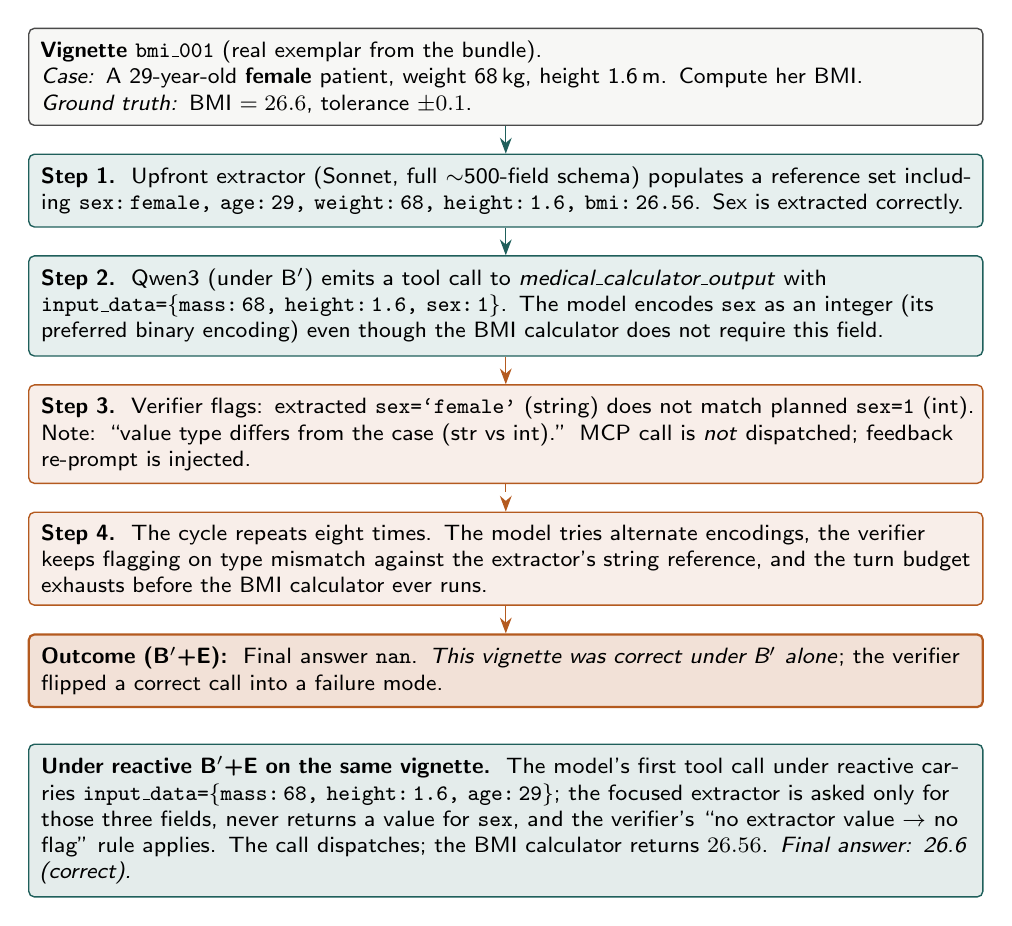
\begin{tikzpicture}[
  font=\sffamily\footnotesize,
  >={Stealth[length=2.0mm]},
  every node/.style={align=left},
  node distance=3.5mm,
  stepbox/.style={rectangle, rounded corners=2pt, line width=0.5pt,
               inner sep=4.5pt, text width=118mm},
  case/.style={stepbox, draw=warmGray, fill=paleGray},
  primary/.style={stepbox, draw=accent, fill=accentLight},
  verifier/.style={stepbox, draw=condBprimeE, fill=condBprimeE!10},
  bad/.style={stepbox, draw=condBprimeE, fill=condBprimeE!18, line width=0.8pt},
  good/.style={stepbox, draw=condReactive, fill=condReactive!12},
]

\node[case] (case) {%
  \textbf{Vignette \texttt{bmi\_001}} (real exemplar from the bundle).\\
  \textit{Case:} A 29-year-old \textbf{female} patient, weight 68\,kg,
  height 1.6\,m. Compute her BMI.\\
  \textit{Ground truth:} BMI $= 26.6$, tolerance $\pm 0.1$.};

\node[primary, below=of case] (s1) {%
  \textbf{Step 1.}\ \ Upfront extractor (Sonnet, full $\sim$500-field
  schema) populates a reference set including \texttt{sex:\,female,
  age:\,29, weight:\,68, height:\,1.6, bmi:\,26.56}. Sex is extracted
  correctly.};

\node[primary, below=of s1] (s2) {%
  \textbf{Step 2.}\ \ Qwen3 (under B$'$) emits a tool call to
  \toolname{medical\_calculator\_output} with
  \texttt{input\_data=\{mass:\,68, height:\,1.6, sex:\,1\}}. The model
  encodes \texttt{sex} as an integer (its preferred binary encoding)
  even though the BMI calculator does not require this field.};

\node[verifier, below=of s2] (s3) {%
  \textbf{Step 3.}\ \ Verifier flags: extracted \texttt{sex=`female'}
  (string) does not match planned \texttt{sex=1} (int). Note: ``value
  type differs from the case (str vs int).'' MCP call is \emph{not}
  dispatched; feedback re-prompt is injected.};

\node[verifier, below=of s3] (s4) {%
  \textbf{Step 4.}\ \ The cycle repeats eight times. The model tries
  alternate encodings, the verifier keeps flagging on type mismatch
  against the extractor's string reference, and the turn budget exhausts
  before the BMI calculator ever runs.};

\node[bad, below=of s4] (s5) {%
  \textbf{Outcome (B$'$+E):}\ \ Final answer \texttt{nan}.
  \emph{This vignette was correct under B$'$ alone}; the verifier
  flipped a correct call into a failure mode.};

\node[good, below=of s5, yshift=-1mm] (s6) {%
  \textbf{Under reactive B$'$+E on the same vignette.}\ \ The model's
  first tool call under reactive carries
  \texttt{input\_data=\{mass:\,68, height:\,1.6, age:\,29\}}; the
  focused extractor is asked only for those three fields, never returns
  a value for \texttt{sex}, and the verifier's ``no extractor value
  $\rightarrow$ no flag'' rule applies. The call dispatches; the BMI
  calculator returns $26.56$. \textit{Final answer: 26.6 (correct).}};

\draw[->, accent]      (case) -- (s1);
\draw[->, accent]      (s1)   -- (s2);
\draw[->, condBprimeE] (s2)   -- (s3);
\draw[->, condBprimeE, dashed] (s3) -- (s4);
\draw[->, condBprimeE] (s4)   -- (s5);

\end{tikzpicture}
\caption{Trace of vignette \texttt{bmi\_001}: an unrequested
\texttt{sex} value in the upfront reference triggers a spurious
flag-loop that reactive extraction avoids.}
\label{fig:loop_trace}
\end{figure}


\Cref{fig:loop_trace} walks through one real exemplar. Under upfront
B$'$+E, the extractor populated a value for \texttt{sex} that the BMI
calculator did not request; the model's tool call used a different
serialization (\texttt{sex=1} vs the extracted \texttt{sex=`female'}),
triggering an unresolvable type-mismatch loop that exhausted the turn
budget. Under reactive extraction the focused prompt for the BMI
calculator did not ask the extractor about \texttt{sex} at all, so no
flag fired and the calculator dispatched cleanly. This is one of 67
vignettes following the recover-by-reactive pattern in our run
(\cref{fig:trajectory_flow}).


\end{document}
